%%%%%%%%%%%%%%%%%%%%%%%%%%%%%%%%%%%%%%%%%%%%%%%%%%%%%%%%%%%%%%%
%  Streamlining Neural Certificate Synthesis  --  Beamer talk
%  (CambridgeUS theme).  Restructured to follow the thesis
%  chapter-for-chapter; slides carry only the visual aids
%  (equations, figures, tables, diagrams) -- details are spoken.
%
%  Build (from this folder), MiKTeX / no latexmk needed:
%    ./build.ps1        (two pdflatex passes: TOC + logo overlays)
%
%  Figures come from ../Figures ; funder logos from ./logos .
%
%  SPEAKER NOTES live in \note{...} and are HIDDEN by default.  To show:
%    uncomment \setbeameroption{show notes} .
%%%%%%%%%%%%%%%%%%%%%%%%%%%%%%%%%%%%%%%%%%%%%%%%%%%%%%%%%%%%%%%
\documentclass{beamer}
\usetheme{CambridgeUS}

\usepackage{amsmath,amssymb,bm}
\usepackage{booktabs}
\usepackage{graphicx}
\usepackage{tikz}
\usetikzlibrary{arrows.meta,positioning,calc,shapes.geometric,fit,backgrounds,decorations.pathreplacing}

% Pull thesis figures and local logos.
\graphicspath{{../Figures/}{logos/}}

% ----- Speaker notes (leave commented to hide) -------------------------------
% \setbeameroption{show notes}

% ----- Palette --------------------------------------------------------------
\definecolor{cSynth}{HTML}{2563EB}   % blue   -- synthesiser / learner
\definecolor{cVerif}{HTML}{059669}   % green  -- sound verifier / safe
\definecolor{cRefut}{HTML}{D97706}   % amber  -- refuter / falsification
\definecolor{cUnsafe}{HTML}{DC2626}  % red    -- unsafe / violation
\definecolor{cUnsure}{HTML}{6B7280}  % grey   -- unsure / abstain
\definecolor{cInk}{HTML}{111827}
\definecolor{cFill}{HTML}{F3F4F6}

% ----- Shared TikZ styles: one clean grammar for every diagram ---------------
%   cbox       = process / actor        (solid rounded rectangle)
%   outputnode = artifact / result      (dotted rounded rectangle)
%   arr        = flow                    (thick arrow)
%   lbl        = edge label              (small, white-backed)
\tikzset{
  >={Stealth[length=2.4mm]},
  font=\sffamily,
  cbox/.style={draw, rounded corners, align=center,
               minimum width=2.1cm, minimum height=0.8cm, font=\scriptsize},
  outputnode/.style={draw, dotted, rounded corners, align=center,
                     minimum width=2.1cm, minimum height=0.8cm, font=\scriptsize},
  arr/.style={->, thick},
  lbl/.style={font=\scriptsize, fill=white, inner sep=1.5pt},
}

\setbeamertemplate{blocks}[rounded][shadow=false]
\setbeamercolor{block title}{bg=blue!10,fg=black}
\setbeamercolor{block body}{bg=gray!10,fg=black}
\setbeamercolor{block title alerted}{bg=red!10,fg=black}
\setbeamercolor{block body alerted}{bg=gray!10,fg=black}
\setbeamercolor{block title example}{bg=green!10,fg=black}
\setbeamercolor{block body example}{bg=gray!10,fg=black}

% ----- Math macros (mirroring the thesis notation) ---------------------------
\DeclareMathOperator*{\argmax}{arg\,max}
\newcommand{\cert}{V}                      % certificate
\newcommand{\drift}{\mathfrak{D}}          % (stochastic) drift
\newcommand{\aX}{\mathcal{X}}              % state space
\newcommand{\aD}{\mathcal{D}}              % counterexample set
\newcommand{\expe}{\mathbb{E}}             % expectation
\newcommand{\expectation}{\expe_{x' \sim P(\cdot \mid x)}[\cert(x')]}
\newcommand{\relu}{\mathrm{ReLU}}
\newcommand{\RN}{\mathbb{R}}
\newcommand{\Diam}{\mathrm{Diam}}
\newcommand{\learner}{\mathrm{Learner}}
\newcommand{\verifier}{\mathrm{Verifier}}
\newcommand{\refuter}{\mathrm{Refuter}}

% ----- Title -----------------------------------------------------------------
\title[Streamlining Neural Certificates]{Streamlining Neural Certificate Synthesis}
\author{William Bailkoski}
\institute[]{\footnotesize Supervisor: Konstantin Kueffner \quad Co-supervisor: Prof.\ Vicen\c{c} G\'omez}
\date{\today}
\titlegraphic{%
  
\includegraphics[height=0.95cm]{everyone.png}\hspace{7mm}%
  
\includegraphics[height=0.95cm]{upf.png}}

\begin{document}

\begin{frame}
  \titlepage
\end{frame}
\logo{}

% \begin{frame}{Outline}
%   \tableofcontents
% \end{frame}

% ===========================================================================
\section{Setup}
% ===========================================================================
\begin{frame}{The verification problem}
  \begin{block}{}\centering
    $\text{system} \models \text{spec}$ \qquad $\forall\ \text{runs satisfy the property}$
  \end{block}
  \begin{itemize}
    \item Continuous state $\aX \subseteq \RN^d$ --- cannot enumerate
    \item Discrete time
    \item \alert{Stochastic}: interested in expected behaviour
    \item Varying degrees of system access
  \end{itemize}
\end{frame}

\begin{frame}{Certificates}
  A certificate $\cert : \aX \rightarrow \RN$ turns a $\forall$-over-trajectories question into a local inequality.\newline

  Different specifications require different certificate types, and different certificate types require different conditions to hold.

  \begin{itemize}
    \item Reachability
    \item Safety
    \item Reach-Avoid
  \end{itemize}

\end{frame}



\begin{frame}{Reaching Great Britain on a stochastic tide}
  \centering
  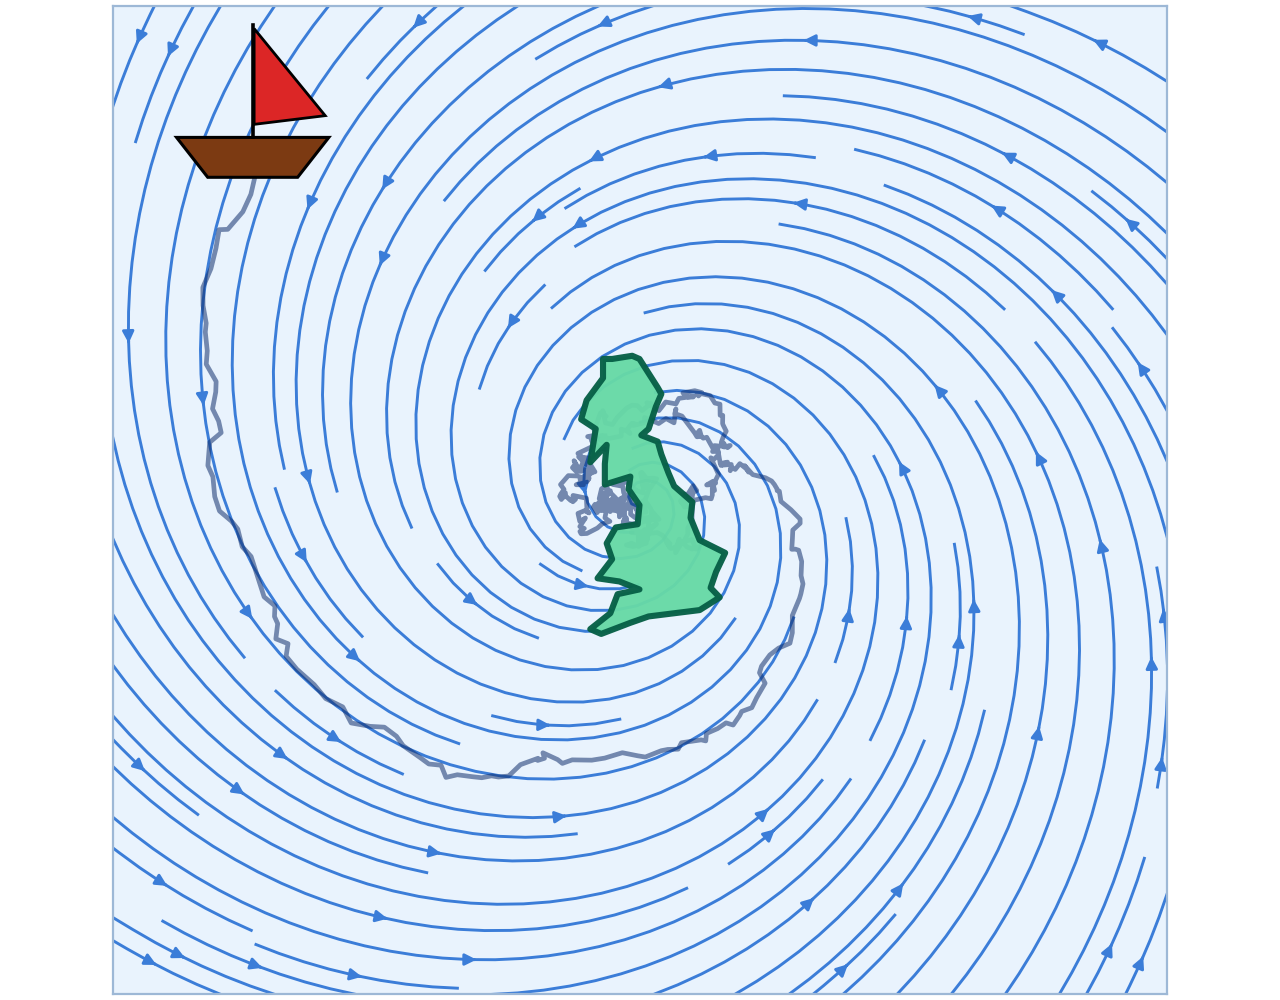
\includegraphics[height=0.66\textheight]{boat_tides_demo.png}\\[2mm]
  {\small Does every path reach \textbf{\color{cVerif}home} in finite expected time?}
  \note{The motivating picture: a boat pushed around by a stochastic tide still reaches home in finite expected time. That reach/termination-in-expectation is exactly what a ranking supermartingale witnesses. Sets up the drift condition on the next slide.}
\end{frame}


\begin{frame}{Certificates}
  A certificate $\cert : \aX \rightarrow \RN$ turns a $\forall$-over-trajectories question into a local inequality.\newline

  Reaching the ``goal'' set in finite expected time is called \emph{termination}.

  \begin{exampleblock}{Ranking supermartingale condition}\centering
    $\drift(x) \;=\; \expe\!\big[\cert(x')\mid x\big] - \cert(x) + \varepsilon \;\le\; 0
     \qquad \forall x \in \aX$
  \end{exampleblock}
  \vspace{3mm}
  \centering\large How do we obtain a valid $\cert$?
\end{frame}

\begin{frame}{CEGIS: synthesise certificates from data}
  \centering
  Learn $\cert$ as a neural network; a sound verifier checks $\forall x$ and
  returns counterexamples to retrain.
  \vspace{5mm}

  \resizebox{0.9\textwidth}{!}{%
  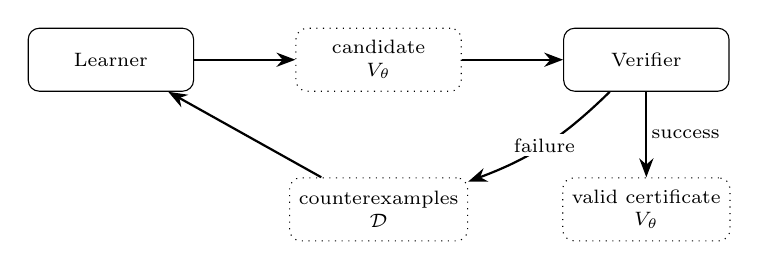
\begin{tikzpicture}
      \node[cbox] (learner) at (0,0) {$\learner$};
      \node[outputnode] (candidate) at (3.4,0) {candidate\\$\cert_\theta$};
      \node[cbox] (verifier) at (6.8,0) {$\verifier$};
      \node[outputnode] (cex) at (3.4,-1.9) {counterexamples\\$\aD$};
      \node[outputnode] (valid) at (6.8,-1.9) {valid certificate\\$\cert_\theta$};
      \draw[arr] (learner) -- (candidate);
      \draw[arr] (candidate) -- (verifier);
      \draw[arr] (verifier) -- node[lbl, right] {success} (valid);
      \draw[arr] (verifier) to[bend left=12] node[lbl, pos=0.5] {failure} (cex);
      \draw[arr] (cex) -- (learner);
  \end{tikzpicture}}
\end{frame}

\begin{frame}{Two goals inside one loop}

  Crucially, there are two distinct jobs:

  \begin{itemize}
    \item Find counterexamples to retrain on (\textbf{\color{cRefut}refutation})
    \item Soundly verify all states (\textbf{\color{cVerif}verification})
  \end{itemize}
  \begin{alertblock}{The bottleneck}\small
    Verification is expensive, yet the verifier does both jobs!
  \end{alertblock}
  \begin{exampleblock}{Hypothesis}\centering\small
    A \textbf{\color{cRefut}cheap refuter} to find counterexamples will reduce reliance on the
    \textbf{\color{cVerif}sound verifier} and speed up the CEGIS pipeline.
  \end{exampleblock}
\end{frame}



% % ===========================================================================
% \section{Benchmarks}
% % ===========================================================================
% \begin{frame}{The Test Suite}
%   \small System characteristics: 
%   \begin{itemize}
%     \item dynamics (function) class: linear, polynomial, transcendental
%     \item noise class: discrete, continuous
%     \item dimension
%   \end{itemize}
%   \begin{table}
%     \centering\small
%     \begin{tabular}{lll}
%       \toprule
%       System & Characteristics \\
%       \midrule
%       $\mathrm{LinSwitch}$  & linear, switched discrete noise, $N$-dim \\
%       $\mathrm{LinStoch}$   & linear, additive noise, $N$-dim \\
%       $\mathrm{DoubleWell}$ & polynomial, additive noise \\
%       $\mathrm{Pendulum}$   & transcendental ($\sin\theta$), controller input $u$ \\
%       \bottomrule
%     \end{tabular}
%   \end{table}
% \end{frame}


% ===========================================================================
\section{Verification}
% ===========================================================================


\begin{frame}{Symbolic solvers}
  \begin{itemize}
    \item Strong \textbf{white-box} assumption
    \item \textbf{Exact} encoding of the dynamics and certificate
    \item \textbf{Non-transcendental} functions only --- no $\sin$, $\tanh$, \ldots
    \item Continuous noise: over-approximate the distribution with \textbf{bins}%
      \footnote{\scriptsize Lechner et al., \emph{Stability Verification in Stochastic Control Systems}, AAAI 2022.}
  \end{itemize}

  \alert{Issues}
  These methods scale poorly with number of variables/constraints to check: dimensionality, noise discretisation, etc. all increase this.
\end{frame}


\begin{frame}{Sampling}
  Minimal \textbf{black-box} assumption: a sample oracle plus a regularity (Lipschitz) bound.
  \vspace{3mm}
  \begin{block}{Confidence bound}\centering
    \[
      \mathrm{CB} \;=\;
      \underbrace{\text{statistical error}}_{\text{\scriptsize$\downarrow$ more samples}}
      \;+\;
      \underbrace{\text{discretisation error}}_{\text{\scriptsize$\downarrow$ refine the grid}}
    \]
  \end{block}
  \vspace{2mm}
  \begin{center}
    upper bound $=$ empirical mean $+\ \mathrm{CB}$\\[1.5mm]
    lower bound $=$ empirical mean $-\ \mathrm{CB}$
  \end{center}
\end{frame}

\begin{frame}{The discretisation error hinges on the Lipschitz constant}
  \begin{block}{Lipschitz constant}\centering
    $\lVert g(x) - g(x')\rVert \;\le\; L_g\,\lVert x - x'\rVert$
  \end{block}
  \begin{block}{}\centering
    discretisation error $=\; L_\drift \cdot \Diam(B)$
  \end{block}
  Two ways to shrink it:
  \begin{itemize}
    \item smaller cells $\rightarrow$ \emph{grid refinement} \hfill (box count $N \approx (L_\drift/\varepsilon)^{d}$)
    \item a \textbf{tighter $L_\drift$} $\rightarrow$ discretise less, everywhere
  \end{itemize}
  \vspace{1mm}
  % \centering\small
  % A tighter $L_\drift$ does for discretisation what more samples do for the statistical error.
\end{frame}




% ===========================================================================
% \section{Advanced Topics in AI}
% ===========================================================================
% (moved to appendix: "Getting L_D" and "Concept: exact L_D")

\begin{frame}{Results: a tighter $L_\drift$}
  \begin{table}
    \centering\small
    \begin{tabular}{cc rrr}
      \toprule
      $d$ & $L_f$ & spectral product & LipBaB & Our method \\
      \midrule
      2 & 0.54 & 1.10 & 0.37 & \textbf{0.27} \\
      2 & 0.60 & 1.60 & 0.52 & \textbf{0.38} \\
      3 & 0.45 & 1.16 & 0.55 & \textbf{0.42} \\
      4 & 0.55 & 1.78 & 0.92 & \textbf{0.60} \\
      4 & 0.51 & 3.11 & 0.94 & \textbf{0.67} \\
      \bottomrule
    \end{tabular}
  \end{table}
  \centering\small
  \textbf{Our method} is $2.7$--$4.6\times$ tighter than the product bound
  ($1.3$--$1.5\times$ tighter than plain LipBaB).\\[1mm]
  Anisotropic per-axis constants then cut the box count by up to $\mathbf{3.5\times}$ in 2D and
  $\mathbf{86\times}$ in 4D.
  % \hfill{\scriptsize(methods in appendix)}
\end{frame}

% (moved to appendix: anisotropic constants)


\begin{frame}{Sample-access verification}
  Two different methods: naive and adaptive.
  \begin{itemize}
    \item Monte Carlo estimation
    \item Adaptive Multi-Armed Bandit
  \end{itemize}

  \alert{Issues}
  Even with adaptive sampling, tighter Lipschitz bounds, and parallelisations we were still unable to get consistent terminations within a $10^9$ sample budget!
\end{frame}





\begin{frame}{Abstract interpretation (bound propagation)}
  State-of-the-art methods via Auto-LiRPA.
  \begin{itemize}
    \item \textbf{IBP} --- cheap, loosest
    \item \textbf{CROWN} --- linear relaxation, keeps neuron correlations
    \item \textbf{$\alpha$-CROWN} --- optimised slopes, tightest, costliest
  \end{itemize}
  \begin{exampleblock}{Anytime}\centering
    Track an upper and lower bound and discretise when the bound straddles zero.
  \end{exampleblock}
\end{frame}

\begin{frame}{CROWN branch-and-bound refines the domain (Pendulum)}
  \centering
  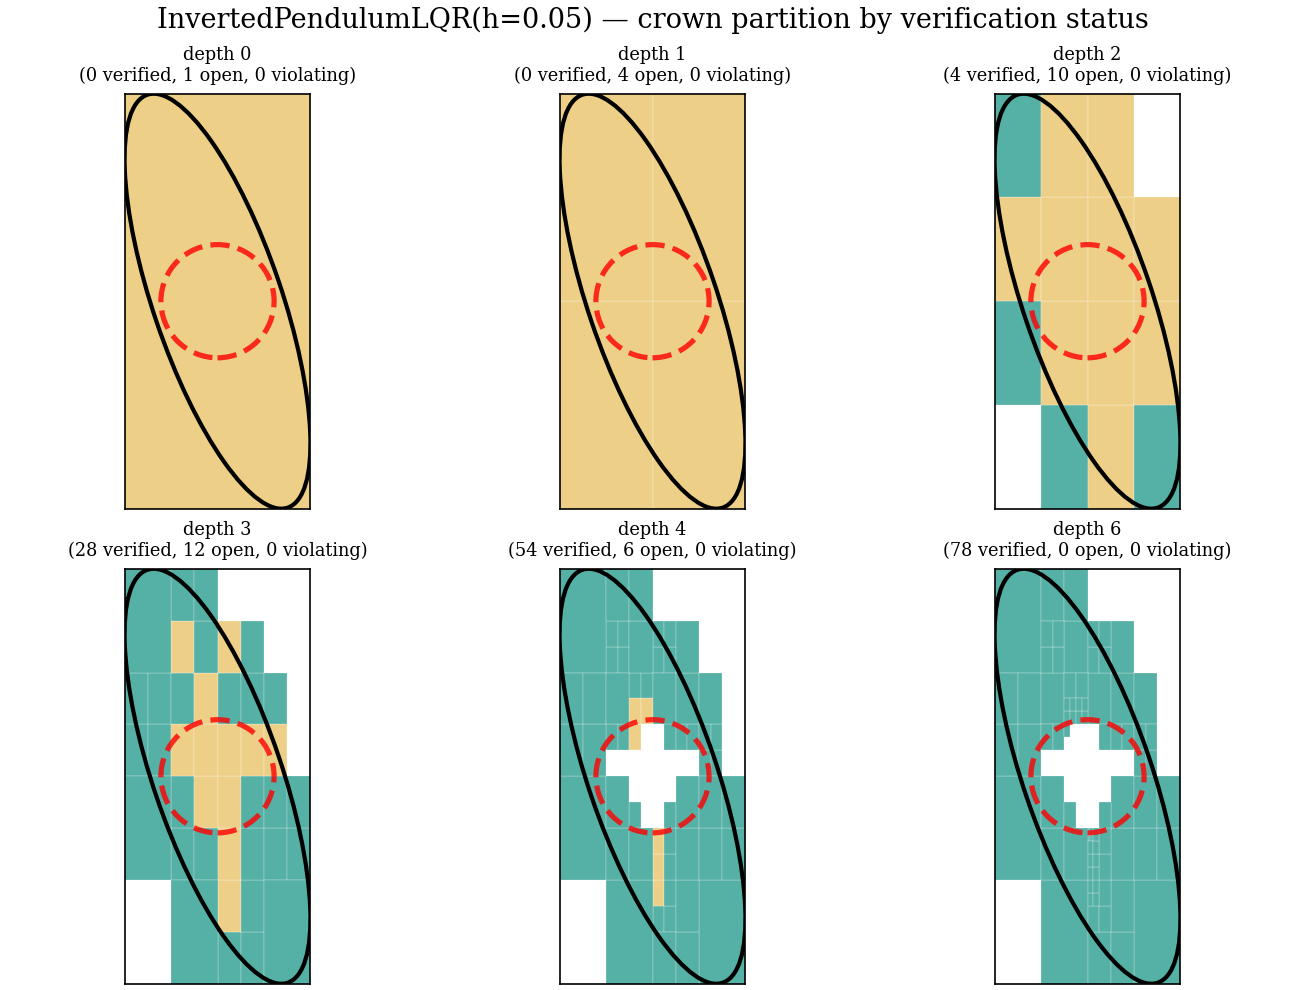
\includegraphics[width=0.95\textwidth,height=0.84\textheight,keepaspectratio]{pendulum_lqr_crown_grid.png}
\end{frame}


% \begin{frame}{Three verifier families}

%   In summary, verifiers are the sound methods of certificate checking. They check the entire domain and return counterexamples.

%   \begin{block}{Symbolic}\small
%     Encode exactly $\rightarrow$ white-box.
%   \end{block}
%   \begin{block}{Abstract interpretation}\small
%     Sound over-approximation through the graph; tune tightness vs.\ speed.
%   \end{block}
%   \begin{block}{Sampling}\small
%     Point evaluations $\Rightarrow$ black-box dynamics; probabilistic guarantee.
%   \end{block}
% \end{frame}

% ===========================================================================
\section{Refutation}
% ===========================================================================


\begin{frame}{Optimisation perspective}
  \begin{block}{Worst-case drift}\centering
    $x^\star \in \argmax_{x \in \aX}\ \drift(x)$
  \end{block}
  \begin{columns}[T]
    \begin{column}{0.5\textwidth}
      \begin{exampleblock}{Verification}\centering
        $\drift(x^\star) \le 0$\\[1mm]
        \scriptsize a $\forall$ claim --- sound, expensive
      \end{exampleblock}
    \end{column}
    \begin{column}{0.5\textwidth}
      \begin{alertblock}{Refutation}\centering
        any $\drift(x) > 0$\\[1mm]
        \scriptsize an $\exists$ witness --- a search problem
      \end{alertblock}
    \end{column}
  \end{columns}
\end{frame}


\begin{frame}{Refutation as black-box optimisation}
  Refuting needs only \emph{some} $x$ with $\drift(x) > 0$ --- an $\exists$, a search problem.
  Soundness not required, so a Monte-Carlo estimate suffices:
  \begin{block}{}\centering
    $\tilde\drift(x) = \dfrac{1}{m}\sum_{i=1}^{m}\cert(f(x,w_i)) - \cert(x) + \varepsilon$
  \end{block}
  \centering\small Run as a cheap \emph{pre-screen}; fall back to the verifier only when it finds nothing.
\end{frame}

\begin{frame}{Six optimisers}
  \begin{columns}[T]
    \begin{column}{0.5\textwidth}
      \textbf{Uninformed}
      \begin{itemize}\small
        \item \textbf{Random} --- quality yardstick
        \item \textbf{Grid} --- non-adaptive
      \end{itemize}
      \textbf{Lipschitz-aware}
      \begin{itemize}\small
        \item \textbf{DIRECT} --- parameter-free
        \item \textbf{AdaLIPO} --- online $L$
      \end{itemize}
    \end{column}
    \begin{column}{0.5\textwidth}
      \textbf{Local / population}
      \begin{itemize}\small
        \item \textbf{Hill climbing} --- gradient $+$ restarts
        \item \textbf{Whale (WOA)} --- population, spiral search
      \end{itemize}
    \end{column}
  \end{columns}
\end{frame}

% \begin{frame}{Tuning on BBOB: whale dominates}
%   Tuned each on 5 BBOB landscapes, scored by normalised regret.
%   \begin{itemize}
%     \item informed methods beat the uninformed ones by 1--5 orders of magnitude
%     \item \alert{whale}: near-zero regret in \emph{milliseconds} --- dominates the fast-and-accurate frontier
%   \end{itemize}
% \end{frame}

\begin{frame}{BBOB: quality versus wall-clock cost}
  \centering
  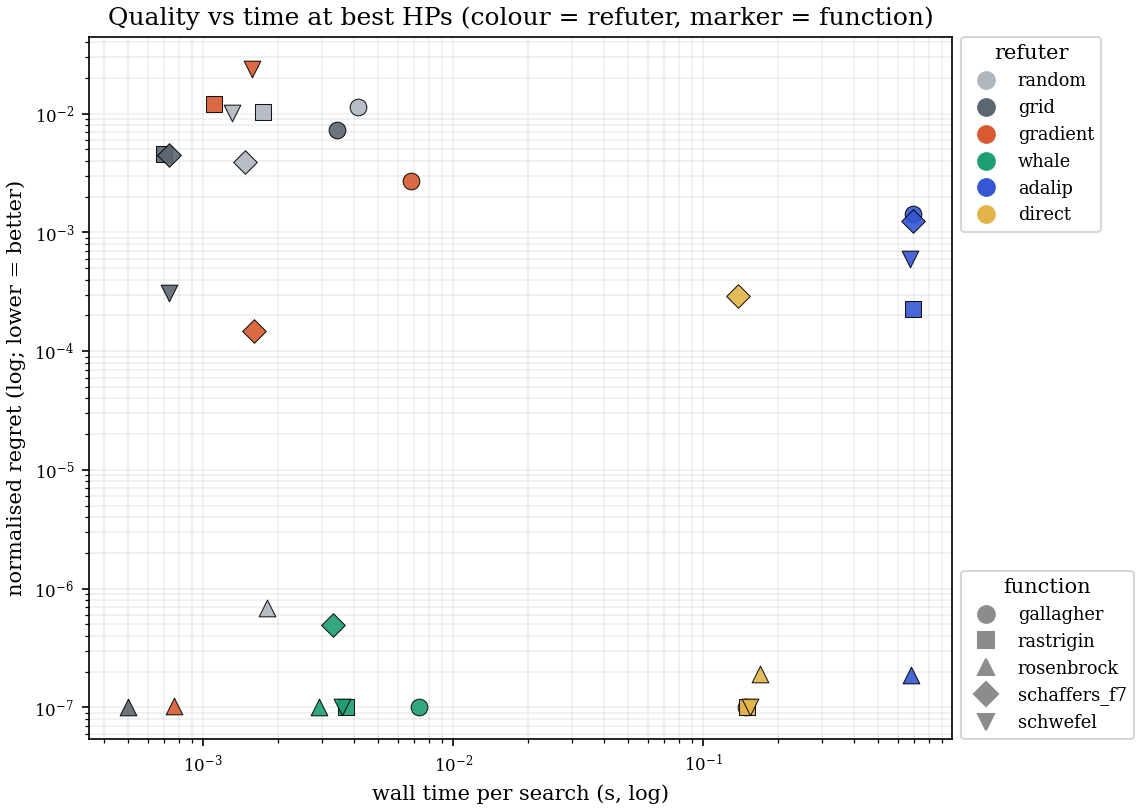
\includegraphics[width=0.95\textwidth,height=0.84\textheight,keepaspectratio]{bbob_quality_vs_time.png}
\end{frame}

\begin{frame}{Refuting faux certificates}
  Replay $2169$ verifier-rejected candidates against the verifier that rejected each.
  \begin{table}
    \centering\small
    \begin{tabular}{lrrr}
      \toprule
      Refuter & Found & Speed-up & Quality \\
      \midrule
      Whale         & $99\%$ & $131\times$ & \textbf{0.049} \\
      AdaLIPO       & $95\%$ & $69\times$  & 0.042 \\
      Random        & $94\%$ & $344\times$ & 0.039 \\
      Grid          & $94\%$ & $352\times$ & 0.038 \\
      Hill climbing & $91\%$ & $262\times$ & 0.038 \\
      DIRECT        & \alert{$40\%$} & $116\times$ & 0.024 \\
      \bottomrule
    \end{tabular}
  \end{table}
  \centering\scriptsize Median $1$--$21$\,ms vs the verifier's $0.48$\,s.
\end{frame}

% \begin{frame}{Faux certificates: reliability and speed-up}
%   \centering
%   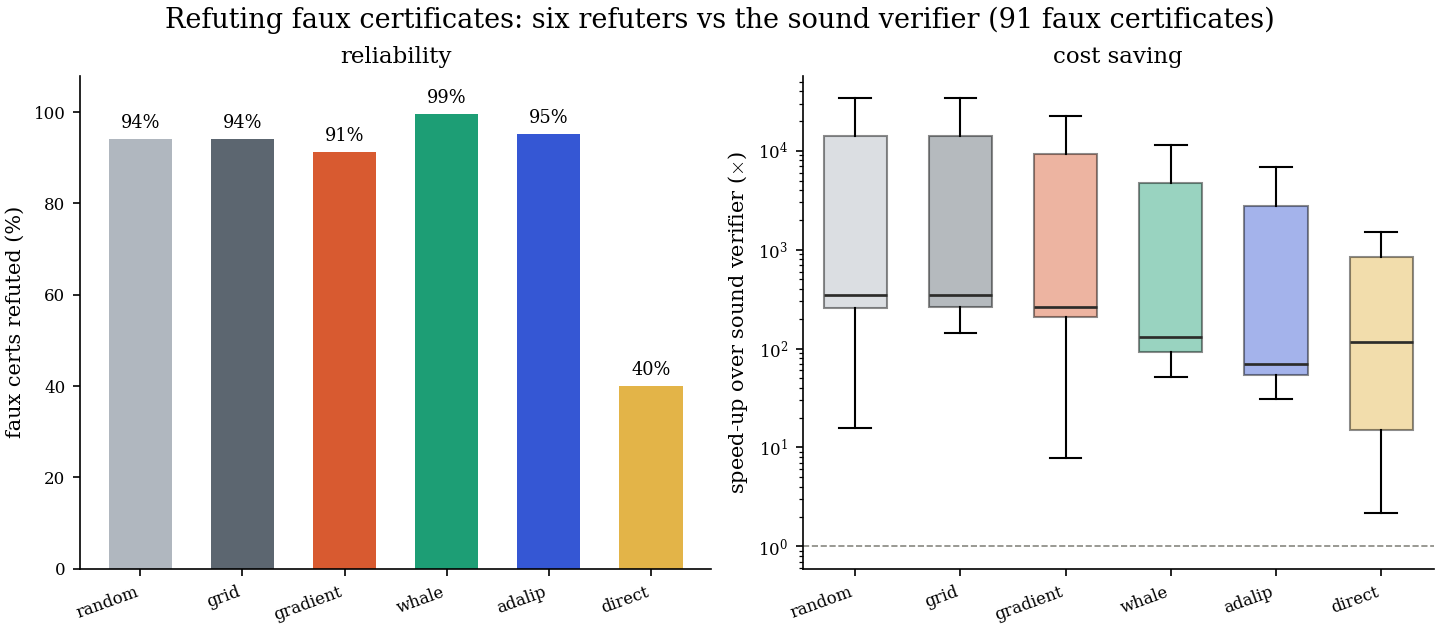
\includegraphics[width=0.95\textwidth,height=0.84\textheight,keepaspectratio]{faux_certs.png}
% \end{frame}

% ===========================================================================
\section{Streamlining CEGIS}
% ===========================================================================
\begin{frame}{The refuter pre-screen}
  \centering
  The cheap refuter hunts first; the sound verifier runs only on a clean candidate.
  \vspace{4mm}

  \resizebox{0.98\textwidth}{!}{%
  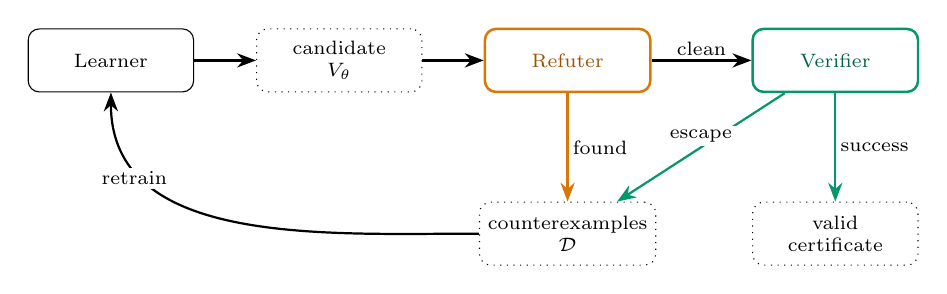
\begin{tikzpicture}[every node/.style={inner sep=3pt}]
    \node[cbox] (learner) at (0,0) {$\learner$};
    \node[outputnode] (cand) at (2.9,0) {candidate\\$\cert_\theta$};
    \node[cbox, draw=cRefut, text=cRefut!70!black, line width=0.9pt] (ref) at (5.8,0) {$\refuter$};
    \node[cbox, draw=cVerif, text=cVerif!65!black, line width=0.9pt] (ver) at (9.2,0) {$\verifier$};
    \node[outputnode] (cex)   at (5.8,-2.2) {counterexamples\\$\aD$};
    \node[outputnode] (valid) at (9.2,-2.2) {valid\\certificate};
    \draw[arr] (learner) -- (cand);
    \draw[arr] (cand) -- (ref);
    \draw[arr] (ref) -- node[lbl, above] {clean} (ver);
    \draw[arr, draw=cRefut] (ref) -- node[lbl, right] {found} (cex);
    \draw[arr, draw=cVerif] (ver) -- node[lbl, above, pos=0.5] {escape} (cex);
    \draw[arr, draw=cVerif] (ver) -- node[lbl, right] {success} (valid);
    \draw[arr] (cex) to[out=180, in=-90] node[lbl, below, pos=0.8] {retrain} (learner);
  \end{tikzpicture}}
  \vspace{3mm}

  {\small Most rounds end at the \textbf{\color{cRefut}refuter}; the \textbf{\color{cVerif}verifier} is paid once, on the final clean candidate.}
\end{frame}

% \begin{frame}{Verifier-only vs.\ refuter pre-screen}
%   \centering
%   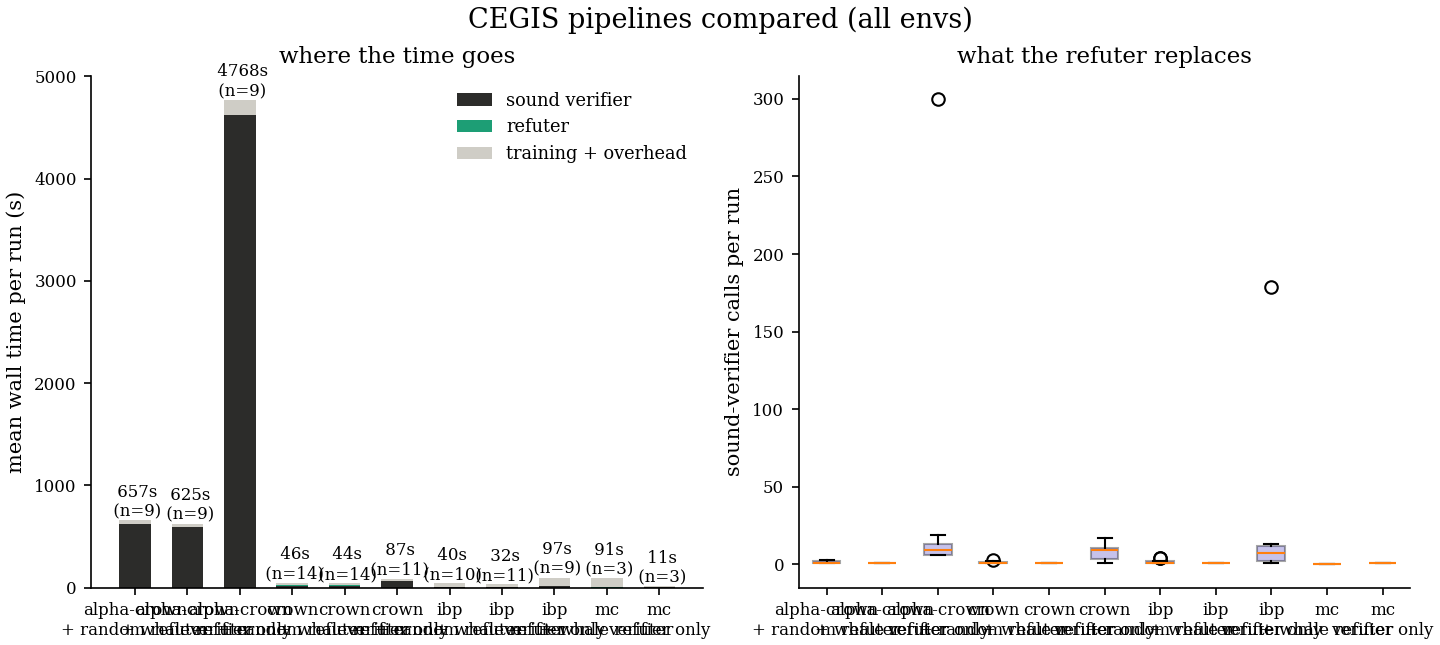
\includegraphics[width=0.95\textwidth,height=0.84\textheight,keepaspectratio]{cegis_pipelines.png}
% \end{frame}


\begin{frame}{Results: speed-up tracks the cost of a sound call}
  \centering\small
  \renewcommand{\arraystretch}{0.95}
  \begin{tabular}{lll rrr r}
    \toprule
    Engine & System & Strategy & Time (s) & Rounds & Calls & Speed-up \\
    \midrule
    CROWN          & LinSwitch & verifier-only & 44.6   & 11.8 & 11.8 & --- \\
                   &           & random        & 52.2   & 15.4 & 2.0  & \alert{$0.85\times$} \\
                   &           & whale         & 38.5   & 10.8 & 1.0  & $1.16\times$ \\
    \midrule
    $\alpha$-CROWN & LinSwitch & verifier-only & 935.0  & 69.2 & 69.2 & --- \\
                   &           & random        & 91.8   & 15.4 & 2.0  & $10.19\times$ \\
                   &           & whale         & 59.6   & 10.8 & 1.0  & \textbf{$15.70\times$} \\
                   & Pendulum  & verifier-only & 9559.4 & 8.0  & 8.0  & --- \\
                   &           & random        & 1363.0 & 6.8  & 1.0  & $5.97\times$ \\
                   &           & whale         & 1331.5 & 8.8  & 1.0  & $6.81\times$ \\
    \bottomrule
  \end{tabular}

  \vspace{2mm}
  \begin{itemize}\small
    \item Expensive calls $\Rightarrow$ big wins ($15.7\times$; Pendulum hours $\to$ minutes)
    \item Cheap calls $\Rightarrow$ little to save --- random can even regress ($0.85\times$)
  \end{itemize}
  \note{Saving = per-call cost times rounds avoided. Skipping sub-second calls buys nothing; skipping 20-minute pendulum calls buys hours.}
\end{frame}

% \begin{frame}{What makes the pre-screen work}
%   \begin{itemize}
%     \item \textbf{Random leaks counterexamples; whale does not} --- exactly one sound call
%     \item \textbf{Counterexample quality matters} --- whale matches the verifier's
%     \item \textbf{Cheapest verifier $\neq$ best} --- whale rescues an IBP $179$-round runaway ($11\times$)
%     \item \textbf{Verification-bound $\to$ training-bound}
%   \end{itemize}
%   \begin{exampleblock}{Recipe}\centering
%     Tightest affordable verifier $+$ a well-tuned refuter pre-screen.
%   \end{exampleblock}
% \end{frame}

% ===========================================================================
\section{Conclusions}
% ===========================================================================
\begin{frame}{Summary \& Contributions}
  \begin{itemize}
    \item \textbf{\color{cVerif}Verifier tool suite} --- a plug-and-play tool for benchmarking CEGIS.
    \item \textbf{\color{cRefut}Refutation as optimisation} --- whale matches verifier quality at $1$--$3$ orders less cost.
    \item \textbf{Central result} --- a refuter pre-screen: up to \textbf{$15.7\times$} faster!
    \item \textbf{\color{cSynth}Lipschitz bounds} --- tighter drift-Lipschitz: $>80\times$ fewer boxes in 4D linear systems.
  \end{itemize}
  \vspace{3mm}
  \centering\small\color{cUnsure}
  Sound verification is the price of a guarantee --- but not every round.
\end{frame}

\begin{frame}{Future work}
  \begin{itemize}
    \item \textbf{Nonlinear drift-Lipschitz} --- bound propagation over $\cert\circ f - \cert$?
    \item \textbf{High-dimension systems} --- can we overcome the curse of dimensionality?
    \item \textbf{Rescue sound sampling} --- Tighter bounds, parallelisations
    \item \textbf{Broader specifications} --- safety, reach-avoid, etc.
    \item \textbf{Abstractions} --- Neural networks are hard to verify by nature
    \end{itemize}
\end{frame}






% =========================================================================




\begin{frame}{}
  \vspace*{1.1cm}
  \centering
  {\Large Thank you}\\[3mm]
  {\small Questions?}\\[7mm]
  {\footnotesize\color{cUnsure}\url{https://github.com/will-bailkoski/streamlining-neural-certificates}}
  \vfill
  
\includegraphics[height=1.0cm]{emai.png}\hspace{9mm}%
  
\includegraphics[height=1.0cm]{eu.png}
  \vspace{4mm}
\end{frame}

% =========================================================================
\appendix
% =========================================================================

\begin{frame}{Getting $L_\drift$}
  \begin{block}{Lipschitz constants compose}\centering
    $L_{f\circ g} \le L_f\,L_g \qquad\quad L_{f\pm g} \le L_f + L_g$
  \end{block}
  \begin{block}{Composition bound \quad($\drift = \cert\circ f - \cert$)}\centering
    $L_\drift \;\le\; L_\cert\,(L_f + 1)$
  \end{block}
  \begin{itemize}
    \item $L_f$ --- \textbf{given} (a property of the dynamics)
    \item $L_\cert$ --- must be estimated from the candidate certificate, \emph{efficiently}
  \end{itemize}
\end{frame}

\begin{frame}{Concept: exact $L_\drift$}
  Assume a linear, deterministic system $A$; compose the drift network
  $\drift = \cert\circ A - \cert$ and run LipBaB over its ReLU regions.
  \begin{block}{Exact drift-Lipschitz constant}\centering
    $L_\drift \;=\; \max\big\{\,\lVert A^{\top} g_j - g_i\rVert \;:\; R_i \cap A^{-1}R_j \cap \aX \neq \emptyset \,\big\}$
  \end{block}
  \begin{itemize}\small
    \item keeps the \textbf{cancellation} between $A^{\top}g_j$ and $g_i$
    \item maximises over regions $i,j$ \textbf{independently}
  \end{itemize}
\end{frame}

\begin{frame}{Anisotropic constants for grid-aligned cells}
  Per-axis sensitivity, free from LipBaB's per-region gradients:
  \[
    L_\cert(e_i) \;=\; \sup_{x}\Big|\tfrac{\partial \cert}{\partial x_i}\Big| \;\le\; L_\cert .
  \]
  \vspace{-2mm}
  \begin{center}On an axis-aligned cell with sides $w_1,\dots,w_d$:\end{center}
  \begin{columns}[c]
    \begin{column}{0.45\textwidth}
      \begin{block}{Isotropic}\centering
        $|\cert(x)-\cert(y)| \le L_\cert\,\lVert w\rVert_2$
      \end{block}
    \end{column}
    \begin{column}{0.45\textwidth}
      \begin{exampleblock}{Anisotropic}\centering
        $\displaystyle |\cert(x)-\cert(y)| \le \sum_i L_\cert(e_i)\,w_i$
      \end{exampleblock}
    \end{column}
  \end{columns}
  \vspace{2mm}
  \begin{exampleblock}{}\centering
    refine per axis $\Rightarrow$ box count $\displaystyle\;\propto \prod_i L_\cert(e_i)\;$ instead of $L_\cert^{\,d}$
    \\[1.5mm]
    Both contributions together: box count down up to $3.5\times$ (2D) and $86\times$ (4D).
  \end{exampleblock}
\end{frame}



\begin{frame}{Benchmark phase portraits}
  \centering
  \begin{columns}[c]
    \begin{column}{0.5\textwidth}\centering
      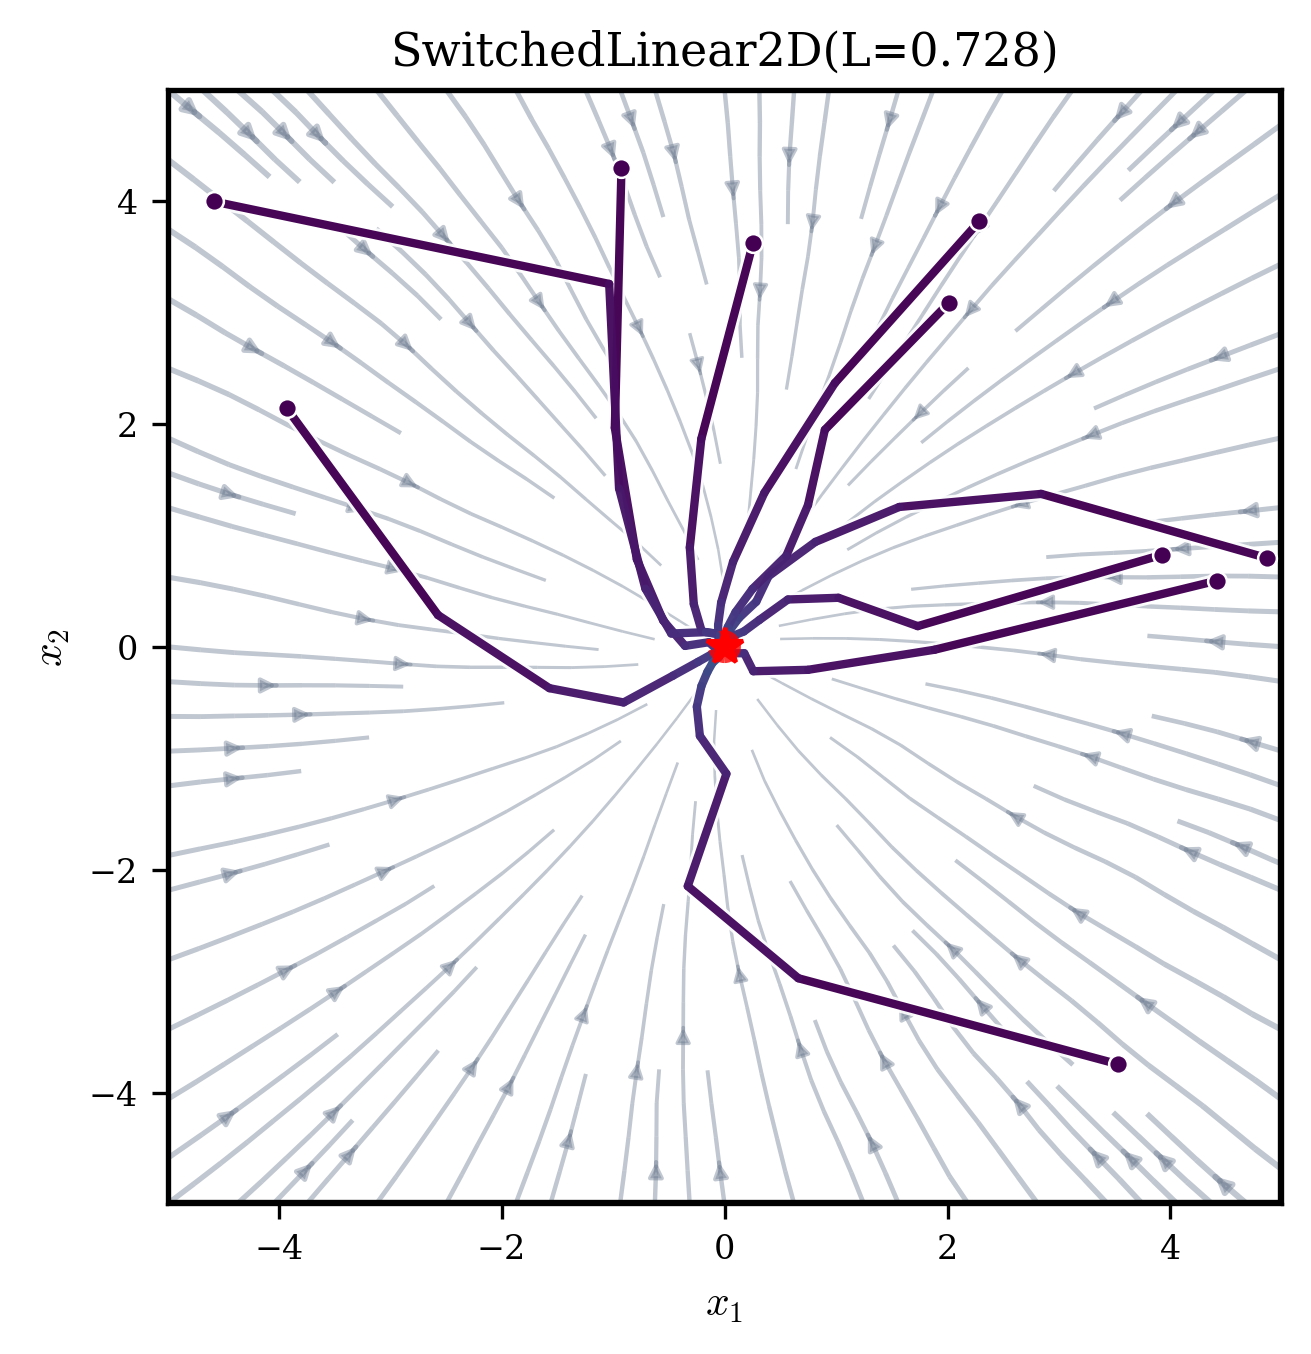
\includegraphics[height=0.34\textheight]{linear2D_phase.png}\\{\scriptsize $\mathrm{LinSwitch}$}\\[1mm]
      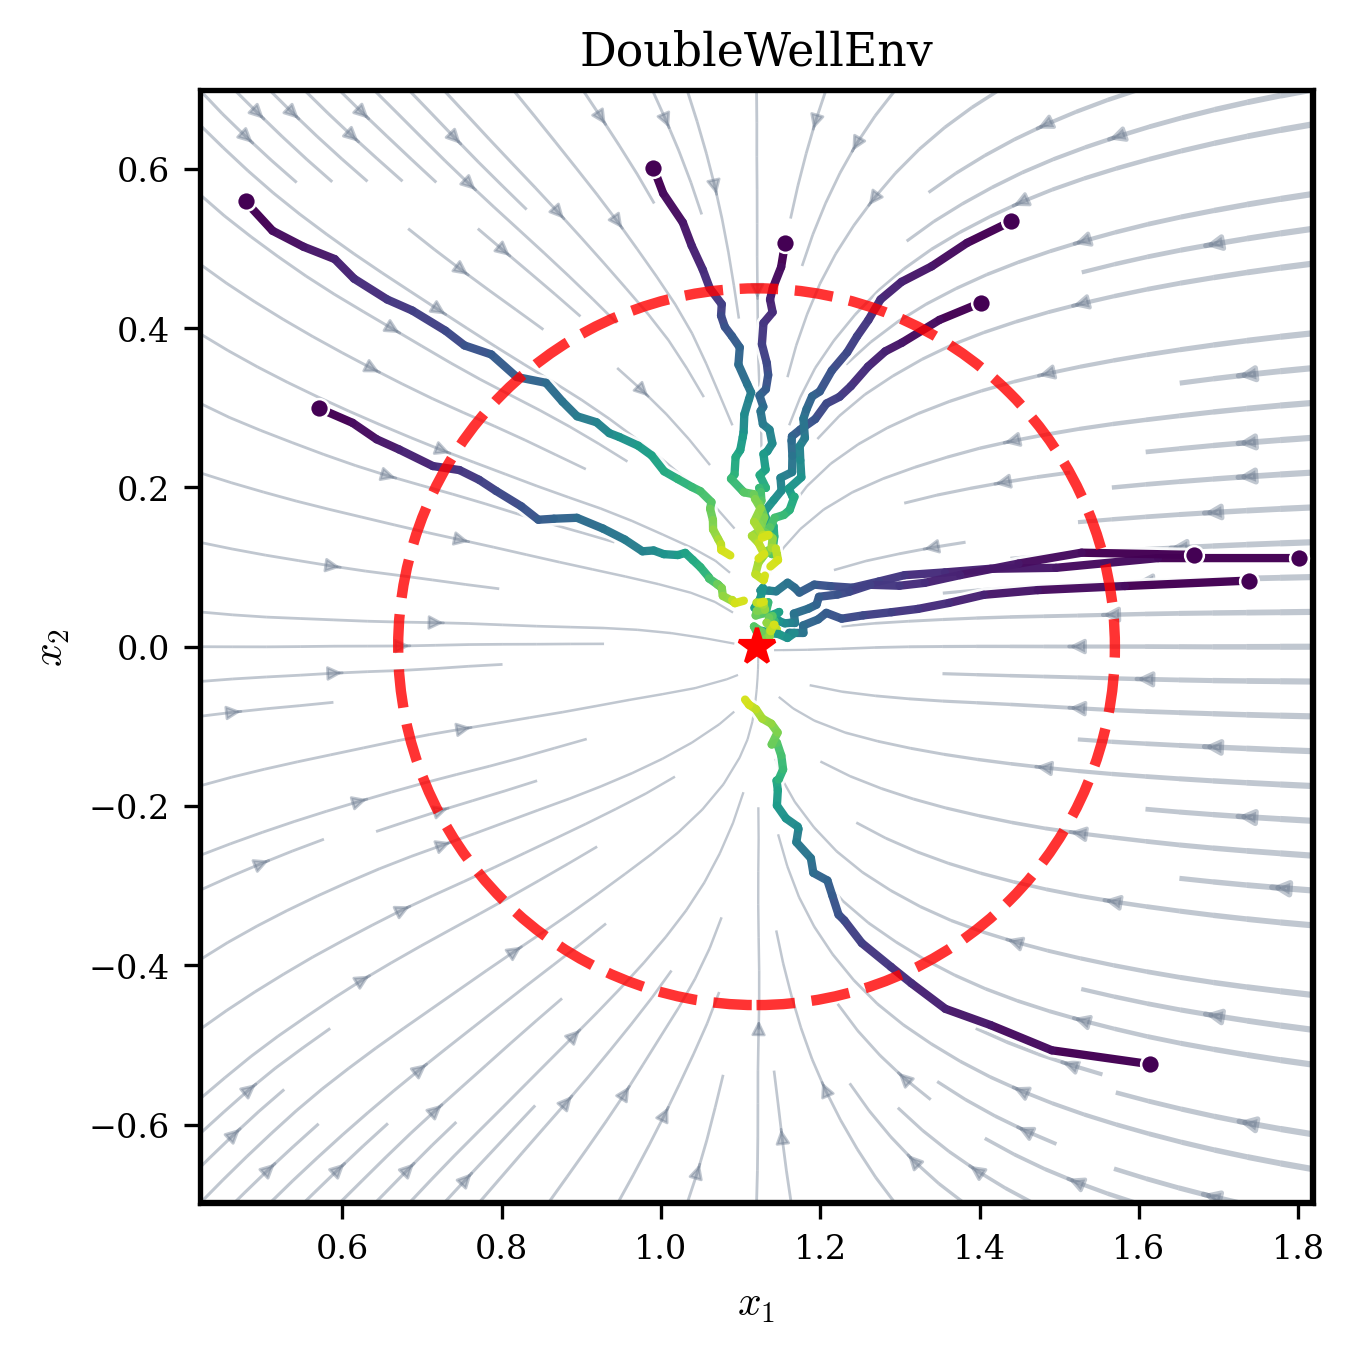
\includegraphics[height=0.34\textheight]{doublewell_phase.png}\\{\scriptsize $\mathrm{DoubleWell}$}
    \end{column}
    \begin{column}{0.5\textwidth}\centering
      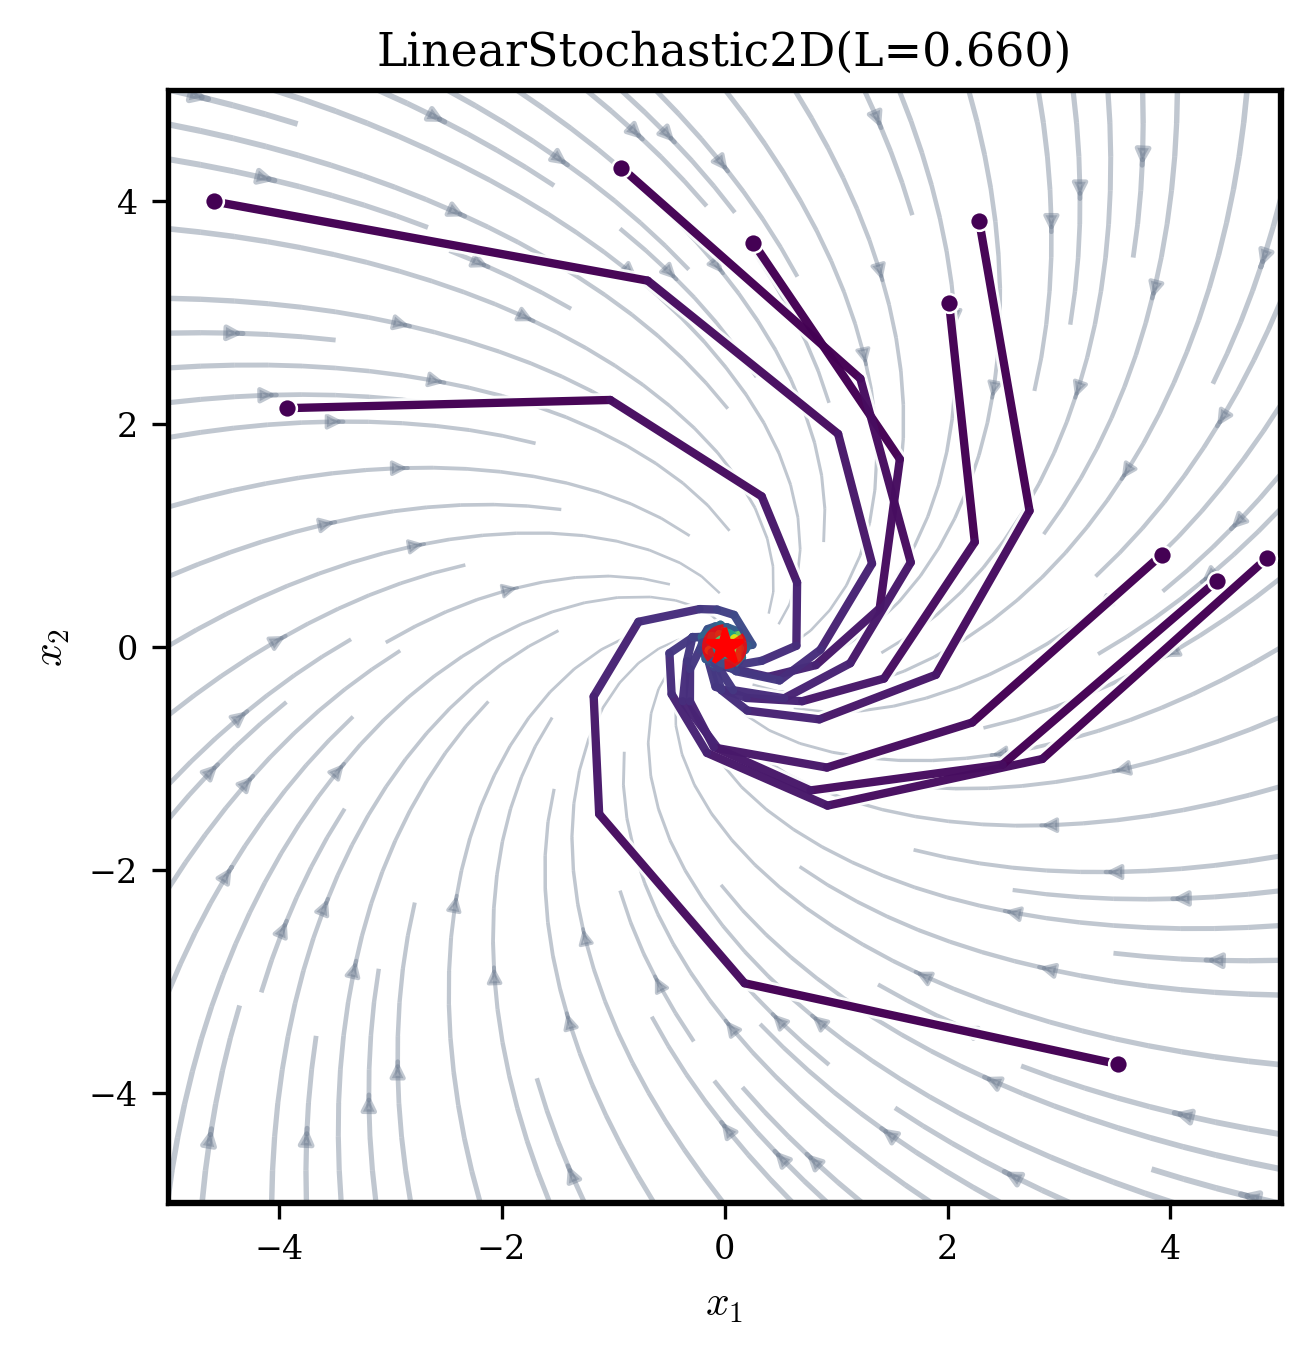
\includegraphics[height=0.34\textheight]{linstoch2D_phase.png}\\{\scriptsize $\mathrm{LinStoch}$}\\[1mm]
      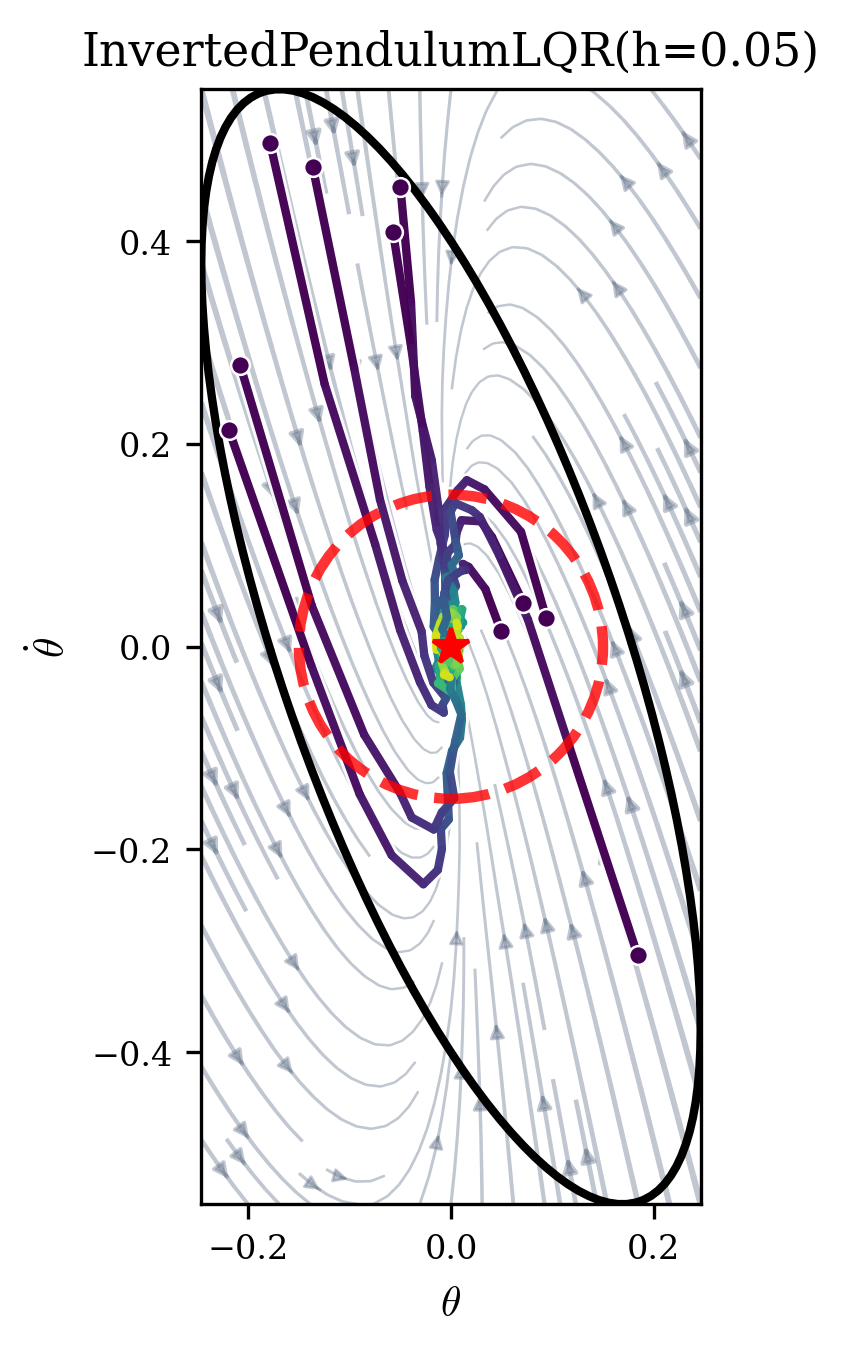
\includegraphics[height=0.34\textheight]{pendulum_lqr_phase.png}\\{\scriptsize $\mathrm{Pendulum}$}
    \end{column}
  \end{columns}
\end{frame}


\begin{frame}{MILP: the noise-discretisation window}
  \centering
  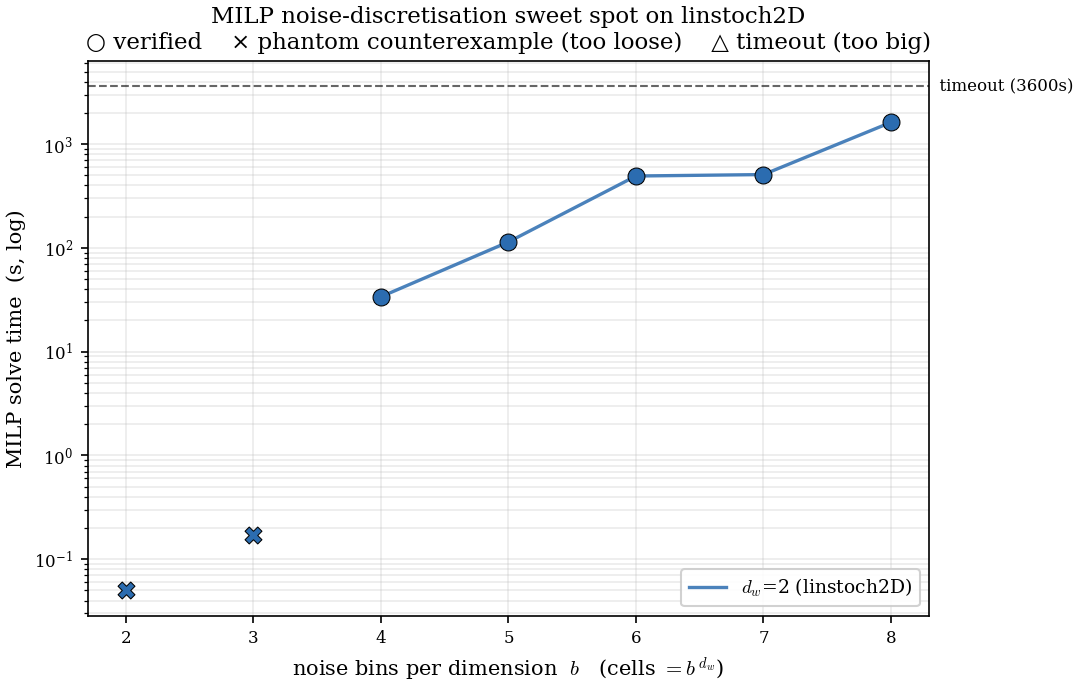
\includegraphics[width=0.95\textwidth,height=0.84\textheight,keepaspectratio]{milp_noise_disc.png}
\end{frame}



\begin{frame}{The capability boundary}
  \begin{table}
    \centering\small
    \begin{tabular}{llccc}
      \toprule
      System & Dynamics & Symbolic & Bound prop. & Sampling \\
      \midrule
      $\mathrm{LinSwitch}$  & linear         & exact$^\ast$ & \checkmark & sound$^\dagger$ \\
      $\mathrm{LinStoch}$   & linear $+$ noise & \textbf{exact only} ($\le$2D) & \alert{fails} & sound$^\dagger$ \\
      $\mathrm{DoubleWell}$ & polynomial     & exact$^\ast$ & \checkmark & sound$^\dagger$ \\
      $\mathrm{Pendulum}$   & transcendental & \alert{abstains} & \textbf{only this family} & sound$^\dagger$ \\
      \bottomrule
    \end{tabular}
  \end{table}
  \vspace{2mm}
  \begin{exampleblock}{}\centering\small
    No single family spans the suite --- the boundary is \emph{two-sided}.\\
    LiRPA drives the campaign; rejected candidates become the \emph{faux-cert} library.
  \end{exampleblock}
  \note{$^\ast$ Z3 sound but returns unknown/timeout in practice. $^\dagger$ sampling sound but not run at full scale. Two takeaways: no universal verifier, and a sound call is fundamentally expensive.}
\end{frame}


% backup: box count now merged into the confidence-bound slides; margin budget is out of the current flow
\begin{frame}{Why it matters for grid verification}
  \begin{columns}[T]
    \begin{column}{0.5\textwidth}
      Grid the domain; each cell needs $L_\drift\cdot\Diam(B) \lesssim \varepsilon$.
      \begin{alertblock}{Box count}\centering
        $N \;\approx\; \Big(\dfrac{L_\drift}{\varepsilon}\Big)^{d}$
      \end{alertblock}
      A $d$-th power of $L_\drift$ --- tightening compounds with dimension.
    \end{column}
    \begin{column}{0.5\textwidth}\centering
      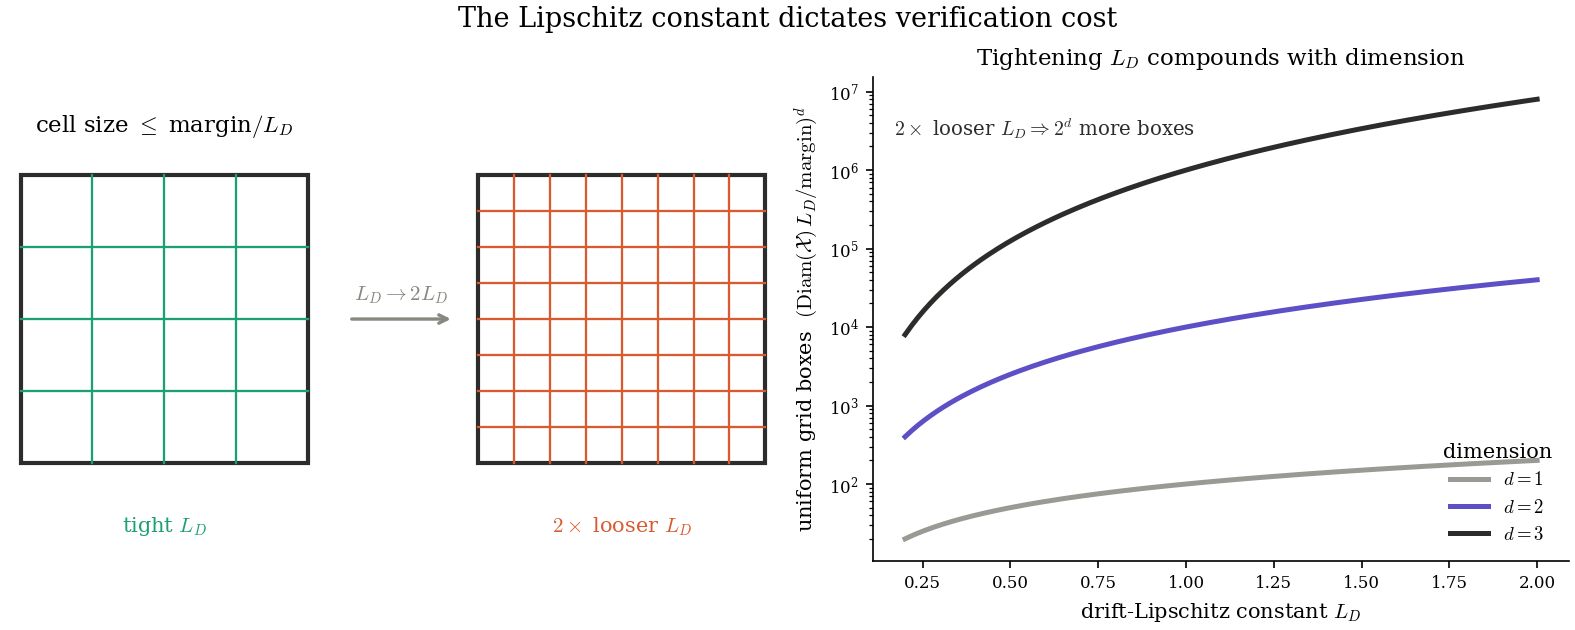
\includegraphics[width=\linewidth]{lipschitz_gridding.png}
    \end{column}
  \end{columns}
\end{frame}

\begin{frame}{The margin budget}
  $L_\cert$ also caps the margin you can certify \emph{at all}:
  \begin{columns}[T]
    \begin{column}{0.54\textwidth}
      \begin{block}{}\centering
        $\varepsilon \;\le\; L_\cert\,\inf_{x}\ \expe_{x'}\!\big[\lVert x - x'\rVert\big]$
      \end{block}
      \small\alert{Danger:} too-small $L_\cert$ (an over-constrained net) makes verification
      \emph{infeasible} --- not just expensive.
    \end{column}
    \begin{column}{0.46\textwidth}\centering
      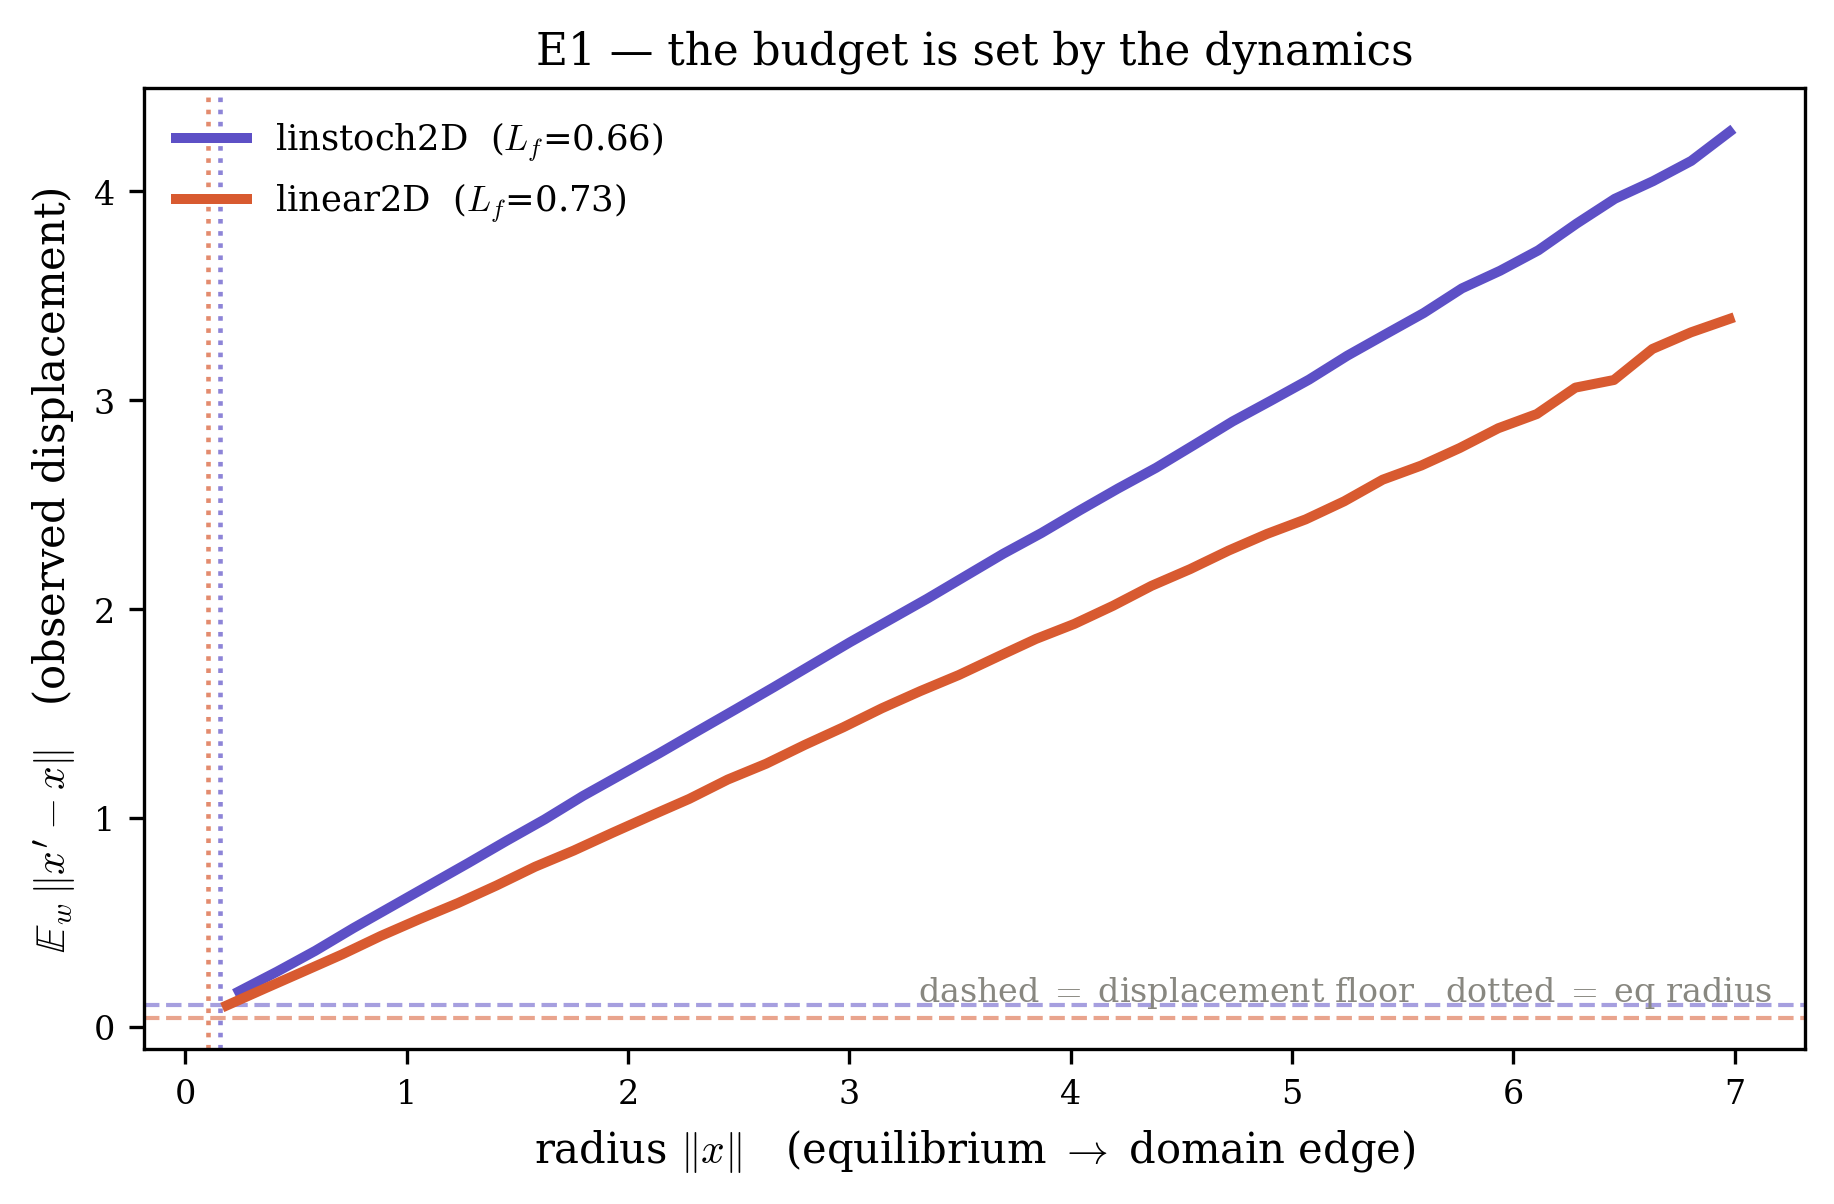
\includegraphics[width=\linewidth]{lipschitz_budget_curve.png}
    \end{column}
  \end{columns}
\end{frame}



\begin{frame}{The product-of-layers bound}
  \centering
  \resizebox{!}{0.5\textheight}{%
  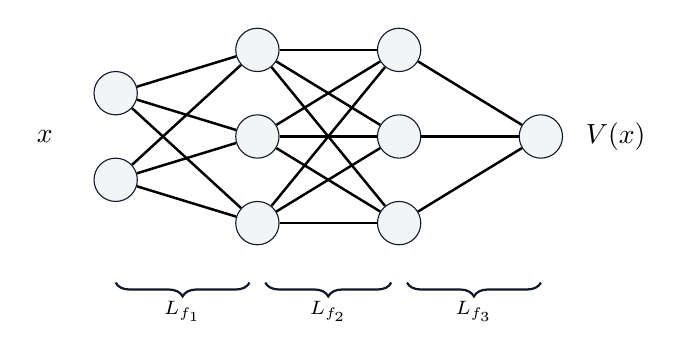
\begin{tikzpicture}[
      neuron/.style={circle, draw=cInk, fill=cFill, minimum size=5.5mm, inner sep=0},
      syn/.style={draw=black, line width=0.9pt},
      brc/.style={decorate, decoration={brace, amplitude=5pt, mirror, raise=3pt}, draw=cInk, thick}
    ]
    % neurons
    \node[neuron] (I1) at (0,0.55) {};
    \node[neuron] (I2) at (0,-0.55) {};
    \node[neuron] (A1) at (1.8,1.1) {};
    \node[neuron] (A2) at (1.8,0) {};
    \node[neuron] (A3) at (1.8,-1.1) {};
    \node[neuron] (B1) at (3.6,1.1) {};
    \node[neuron] (B2) at (3.6,0) {};
    \node[neuron] (B3) at (3.6,-1.1) {};
    \node[neuron] (O)  at (5.4,0) {};
    % synapses (behind neurons)
    \begin{scope}[on background layer]
      \foreach \a in {I1,I2} \foreach \b in {A1,A2,A3} \draw[syn] (\a) -- (\b);
      \foreach \a in {A1,A2,A3} \foreach \b in {B1,B2,B3} \draw[syn] (\a) -- (\b);
      \foreach \b in {B1,B2,B3} \draw[syn] (\b) -- (O);
    \end{scope}
    % in / out
    \node at (-0.9,0) {$x$};
    \node at (6.35,0) {$\cert(x)$};
    % per-layer braces: each layer is one composed function application
    \draw[brc] (0.0,-1.75)  -- (1.7,-1.75)
        node[midway, below=6pt, font=\scriptsize] {$L_{f_1}$};
    \draw[brc] (1.9,-1.75)  -- (3.5,-1.75)
        node[midway, below=6pt, font=\scriptsize] {$L_{f_2}$};
    \draw[brc] (3.7,-1.75)  -- (5.4,-1.75)
        node[midway, below=6pt, font=\scriptsize] {$L_{f_3}$};
  \end{tikzpicture}}

  \vspace{2mm}
  \begin{block}{}\centering
    $\cert = f_l \circ \cdots \circ f_1
     \quad\Longrightarrow\quad
     L_\cert \le \displaystyle\prod_{\ell=1}^{l}L_{f_\ell}$
  \end{block}
\end{frame}



\begin{frame}{The MAB verifier: refine only where it matters}
  \centering
  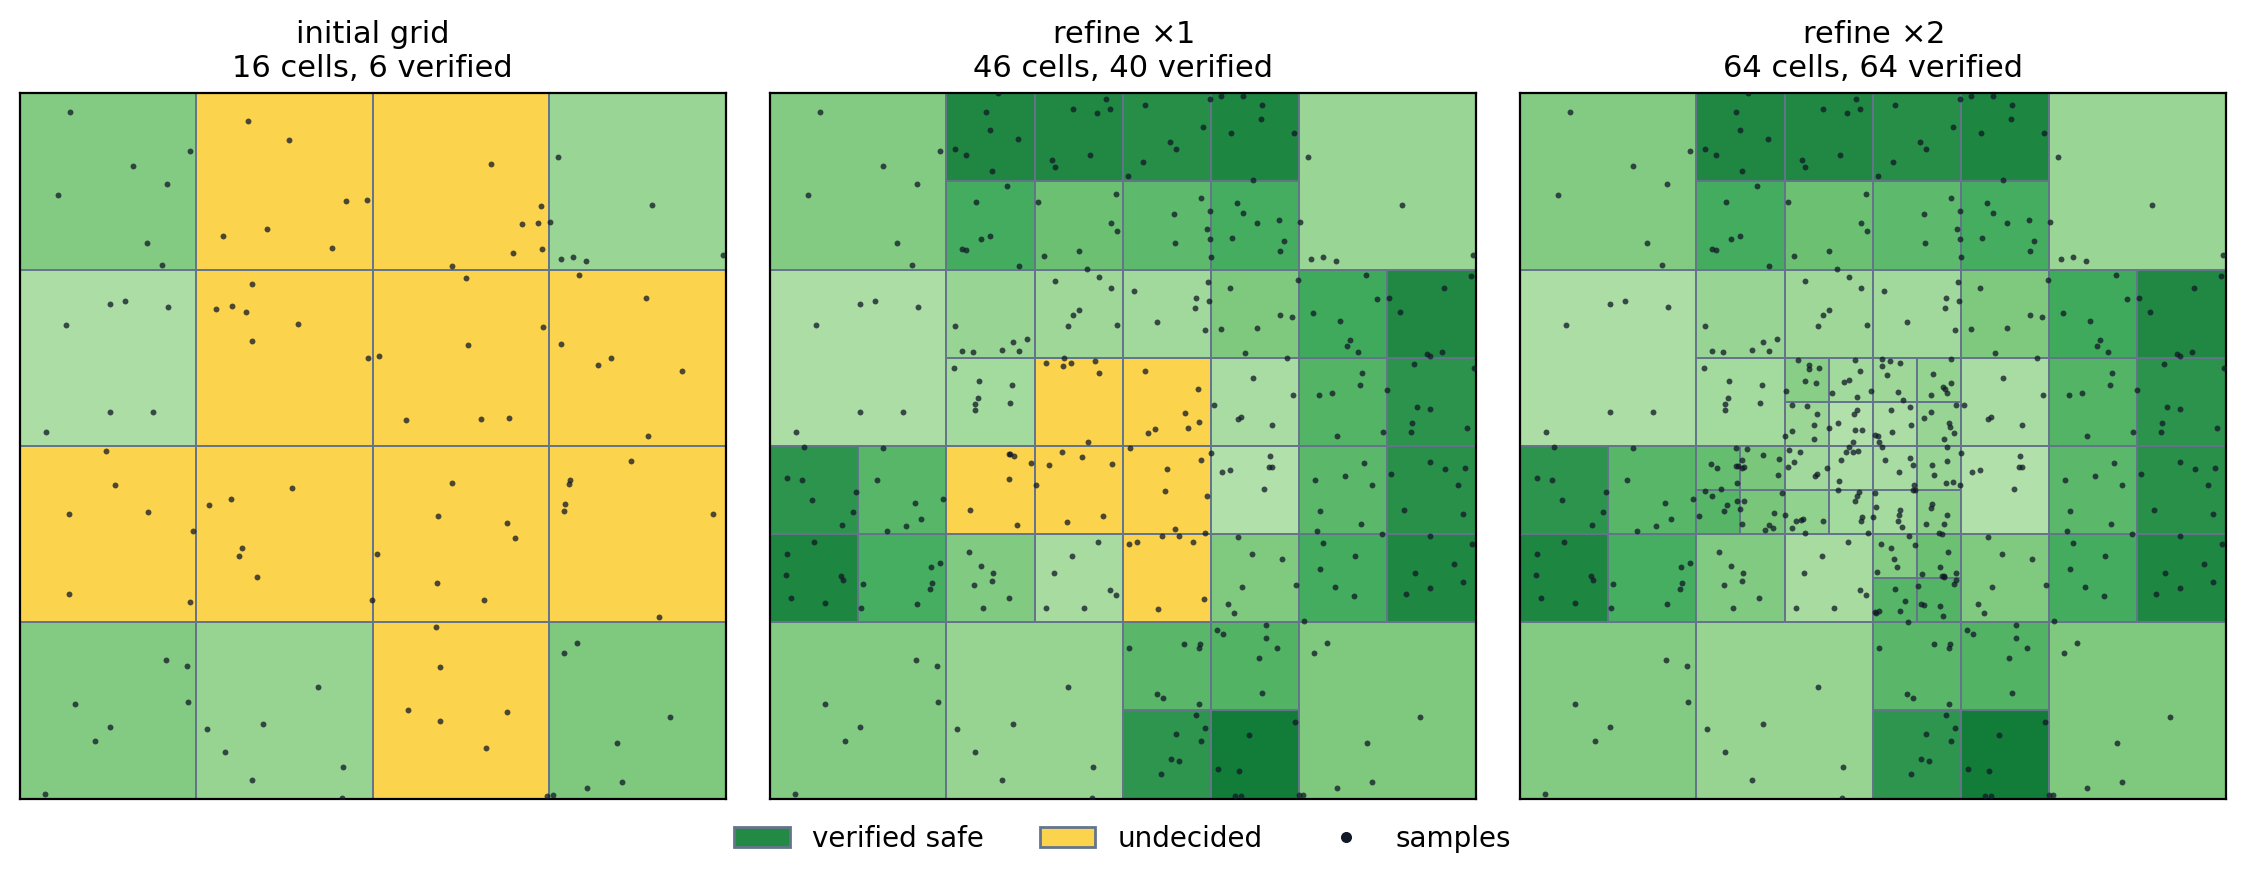
\includegraphics[width=\linewidth]{mab_refine_demo.png}\\[1mm]
  {\small Sample each cell; it \textbf{\color{cVerif}verifies} once its UCB $\le 0$ (greener $=$ safer),
   otherwise it \emph{splits}. Refinement concentrates on the thin-margin core.}
\end{frame}





% ======================= full CEGIS results table =======================
\begin{frame}{Full CEGIS results: IBP \& CROWN}
  \centering\scriptsize
  \renewcommand{\arraystretch}{0.95}
  \begin{tabular}{lll rrr r}
    \toprule
    Engine & System & Strategy & Time (s) & Rounds & Calls & Speed-up \\
    \midrule
    IBP & LinSwitch  & verifier-only & 155.5 & 43.8 & 43.8 & --- \\
        &            & random        & 58.9  & 18.0 & 2.6  & $2.64\times$ \\
        &            & whale         & 39.8  & 10.8 & 1.0  & $3.91\times$ \\
        & DoubleWell & verifier-only & 14.6  & 1.3  & 1.3  & --- \\
        &            & random        & 14.1  & 1.7  & 1.0  & $1.03\times$ \\
        &            & whale         & 18.4  & 2.2  & 1.0  & $1.04\times$ \\
        & Pendulum   & verifier-only & 55.0  & 6.0  & 6.0  & --- \\
        &            & random        & 33.7  & 7.5  & 1.0  & $1.76\times$ \\
        &            & whale         & 57.4  & 10.0 & 1.0  & --- \\
    \midrule
    CROWN & LinSwitch  & verifier-only & 44.6  & 11.8 & 11.8 & --- \\
          &            & random        & 52.2  & 15.4 & 2.0  & \alert{$0.85\times$} \\
          &            & whale         & 38.5  & 10.8 & 1.0  & $1.16\times$ \\
          & DoubleWell & verifier-only & 41.7  & 1.7  & 1.7  & --- \\
          &            & random        & 31.3  & 2.2  & 1.0  & $1.48\times$ \\
          &            & whale         & 32.0  & 2.2  & 1.0  & $1.51\times$ \\
          & Pendulum   & verifier-only & 203.1 & 7.0  & 7.0  & --- \\
          &            & random        & 57.8  & 6.8  & 1.0  & $2.74\times$ \\
          &            & whale         & 66.8  & 8.5  & 1.0  & $3.19\times$ \\
    \bottomrule
  \end{tabular}
\end{frame}

\begin{frame}{Full CEGIS results: $\alpha$-CROWN}
  \centering\small
  \renewcommand{\arraystretch}{1.1}
  \begin{tabular}{lll rrr r}
    \toprule
    Engine & System & Strategy & Time (s) & Rounds & Calls & Speed-up \\
    \midrule
    $\alpha$-CROWN & LinSwitch  & verifier-only & 935.0  & 69.2 & 69.2 & --- \\
                   &            & random        & 91.8   & 15.4 & 2.0  & $10.19\times$ \\
                   &            & whale         & 59.6   & 10.8 & 1.0  & \textbf{$15.70\times$} \\
                   & DoubleWell & \multicolumn{5}{c}{\emph{did not complete}} \\
                   & Pendulum   & verifier-only & 9559.4 & 8.0  & 8.0  & --- \\
                   &            & random        & 1363.0 & 6.8  & 1.0  & $5.97\times$ \\
                   &            & whale         & 1331.5 & 8.8  & 1.0  & $6.81\times$ \\
    \bottomrule
  \end{tabular}
  \vspace{3mm}

  {\footnotesize $\alpha$-CROWN Pendulum: $\sim$20-min sound calls turn a multi-hour verifier-only run into $\sim$22 min.}
\end{frame}

% ======================= appendix figures =======================
\begin{frame}{MILP model size grows as $b^{d_w}$}
  \centering
  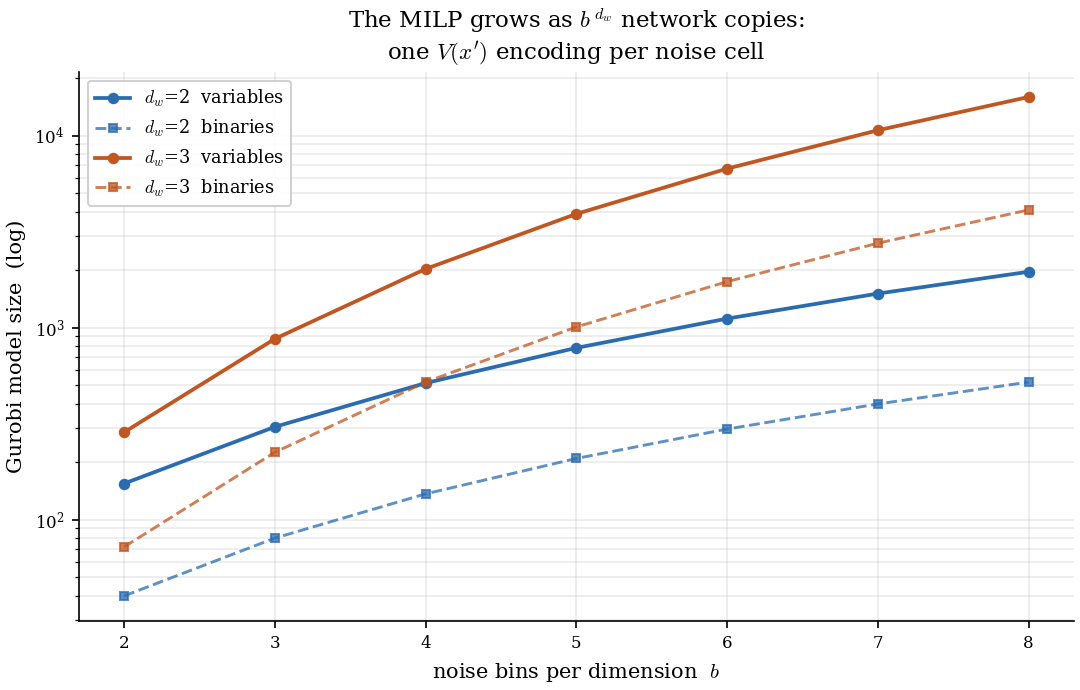
\includegraphics[width=0.9\textwidth,height=0.82\textheight,keepaspectratio]{milp_problem_size.png}
\end{frame}

\begin{frame}{Anytime tightness: IBP / CROWN / $\alpha$-CROWN}
  \centering
  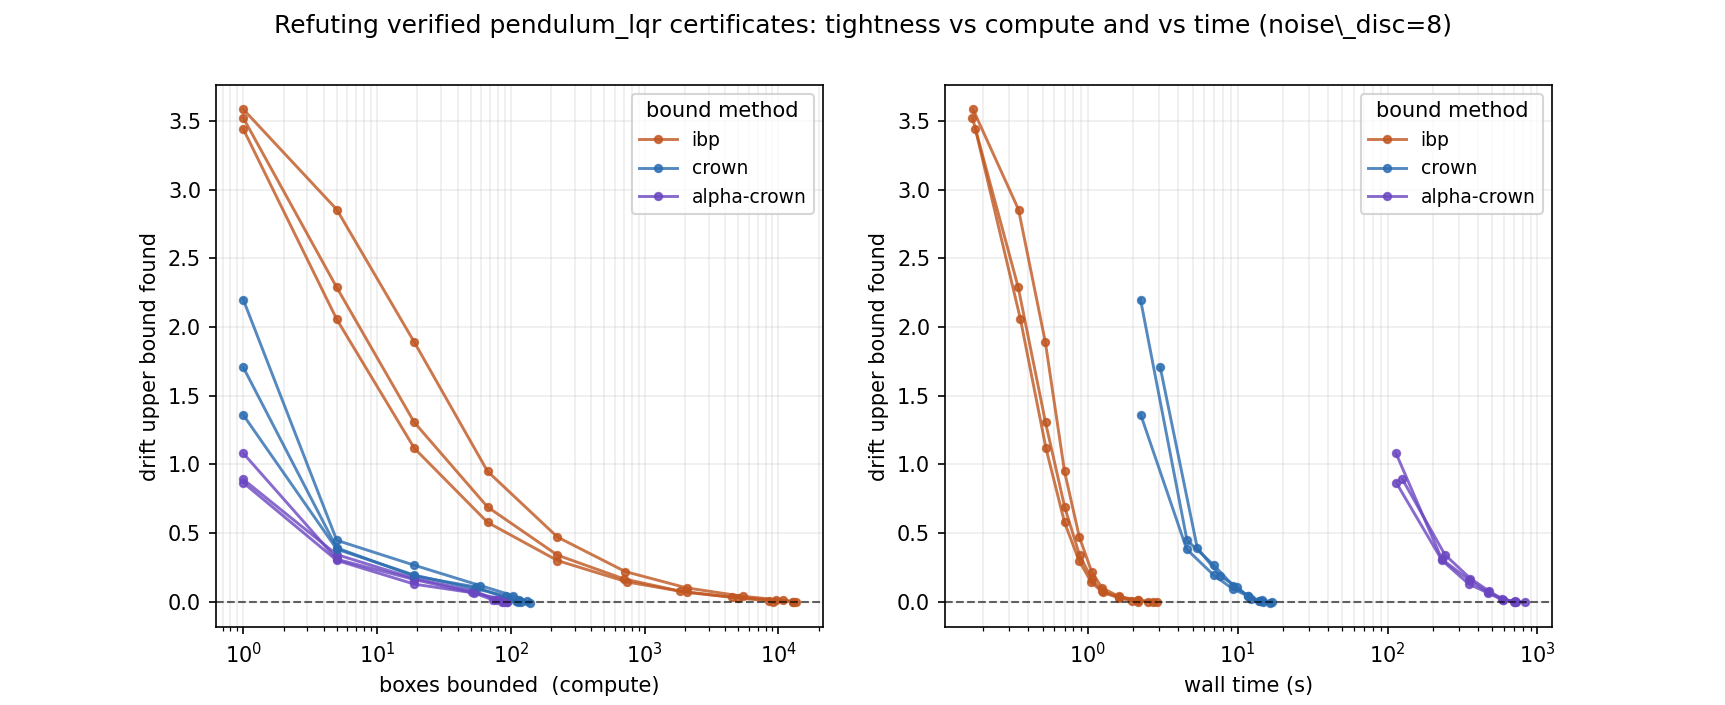
\includegraphics[width=0.98\textwidth,height=0.8\textheight,keepaspectratio]{pendulum_anytime.png}
\end{frame}

\begin{frame}{Sound sampling (MAB): coverage and confidence bounds}
  \centering
  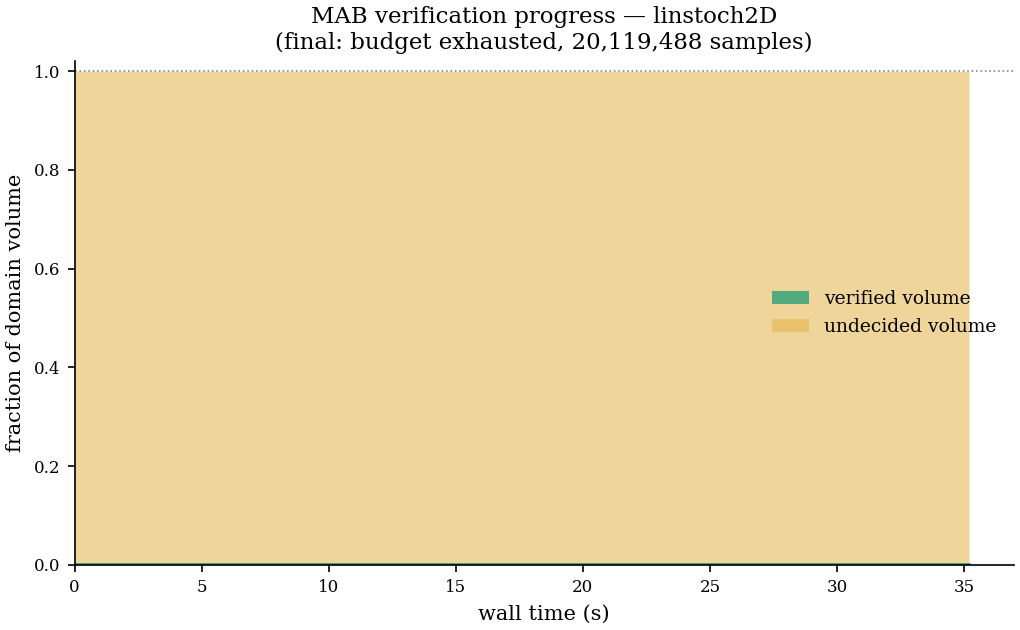
\includegraphics[width=0.49\textwidth,height=0.78\textheight,keepaspectratio]{mab_area.png}\hfill
  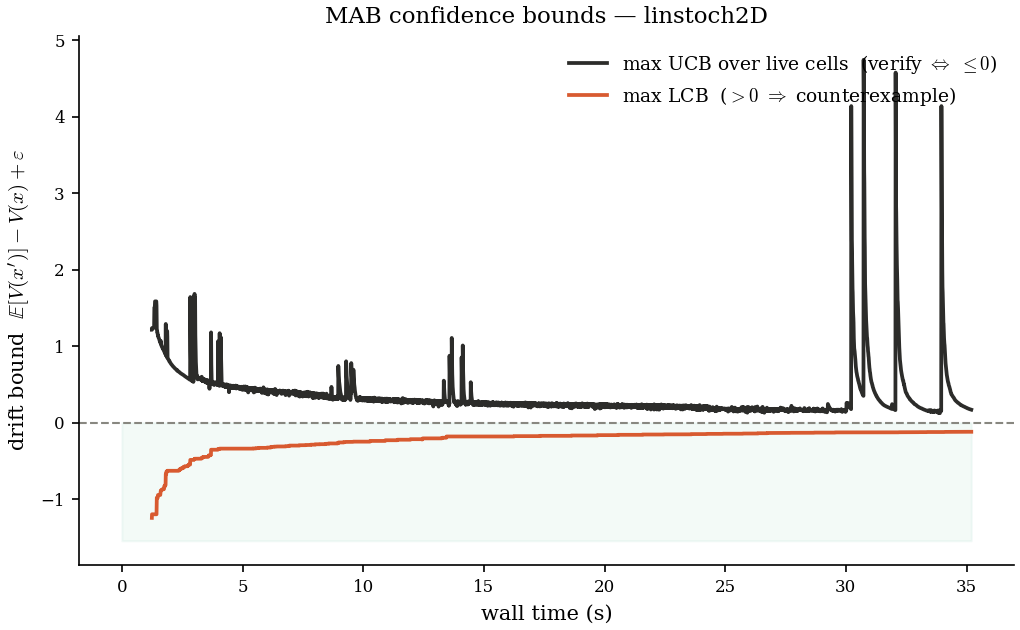
\includegraphics[width=0.49\textwidth,height=0.78\textheight,keepaspectratio]{mab_bounds.png}
\end{frame}

\begin{frame}{Margin budget: demanding more $\varepsilon$ needs a steeper $\cert$}
  \centering
  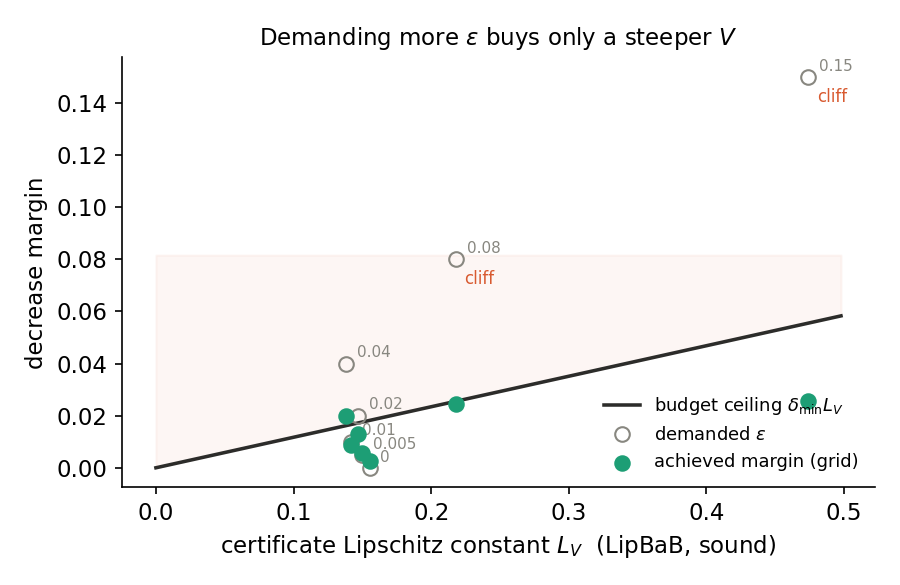
\includegraphics[width=0.85\textwidth,height=0.8\textheight,keepaspectratio]{lipschitz_frontier.png}
\end{frame}

\begin{frame}{Margin-matching: fixed is flat, adaptive tracks the dynamics}
  \centering
  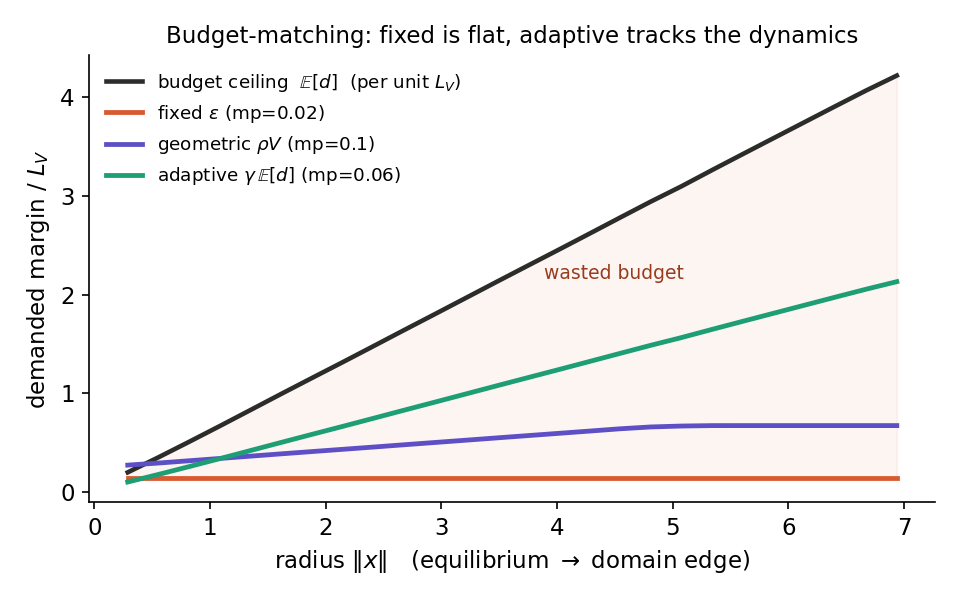
\includegraphics[width=0.85\textwidth,height=0.8\textheight,keepaspectratio]{lipschitz_profiles.png}
\end{frame}

\begin{frame}{The five BBOB test functions}
  \centering
  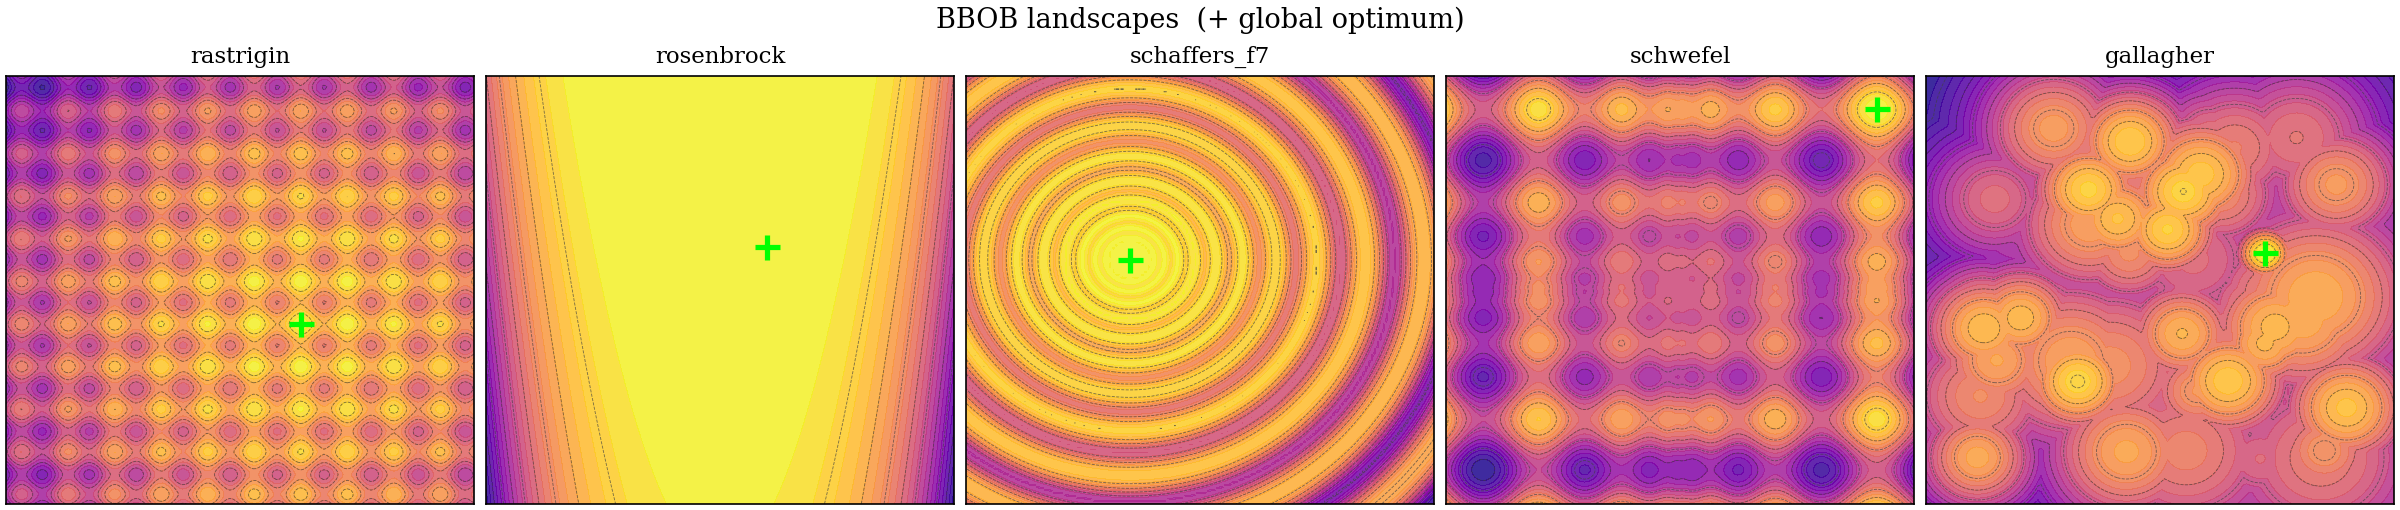
\includegraphics[width=0.98\textwidth,height=0.8\textheight,keepaspectratio]{bbob_landscapes.png}
\end{frame}

\begin{frame}{BBOB: normalised regret per function}
  \centering
  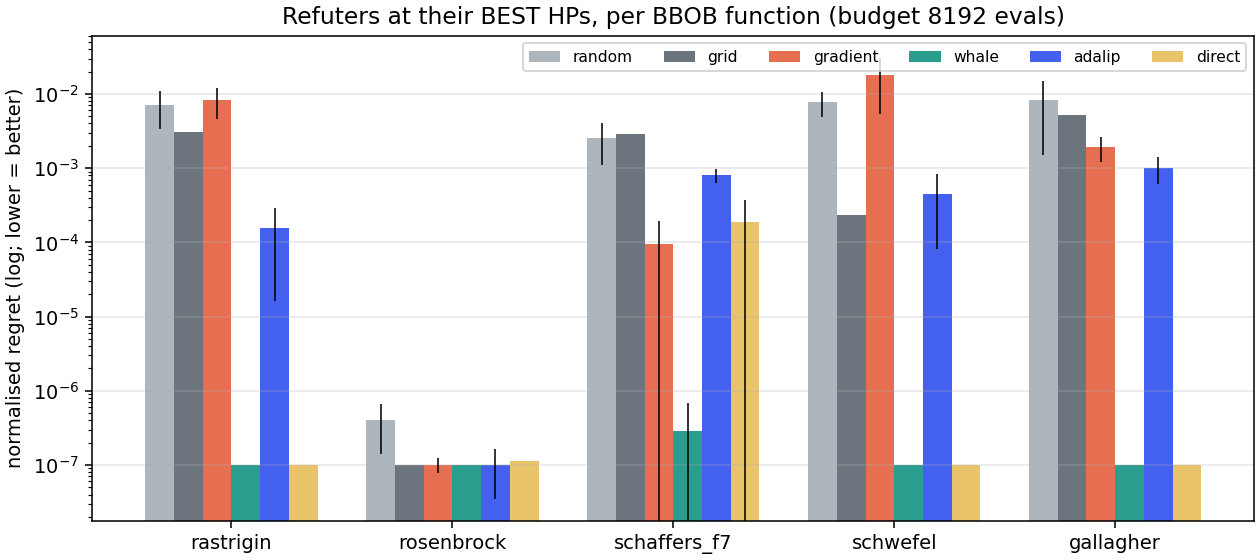
\includegraphics[width=0.96\textwidth,height=0.82\textheight,keepaspectratio]{bbob_quality_per_function.png}
\end{frame}

\begin{frame}{Hyperparameter sweep: regret per combo}
  \centering
  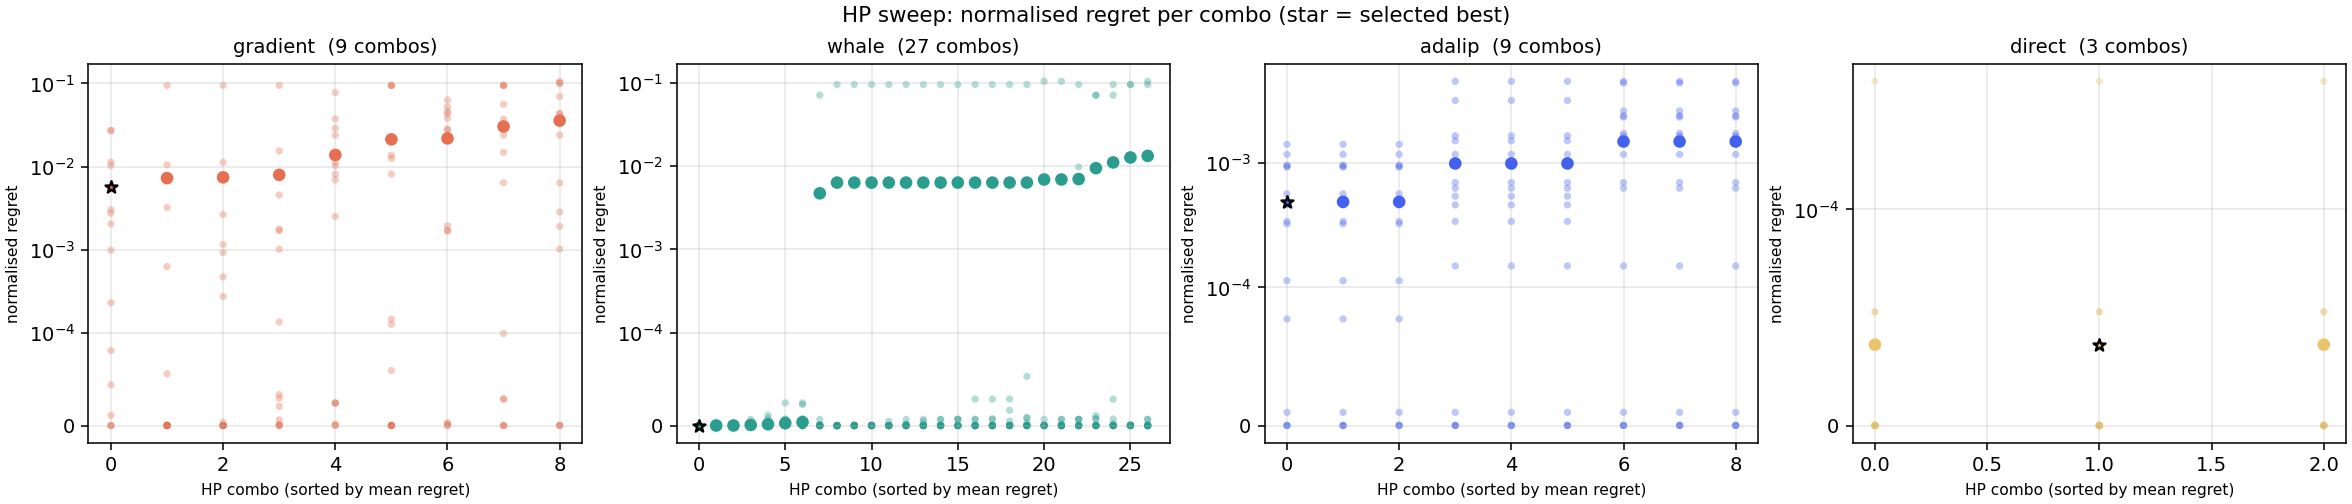
\includegraphics[width=0.98\textwidth,height=0.72\textheight,keepaspectratio]{bbob_hp_sweep.png}
\end{frame}

\begin{frame}{Refuter search patterns (I): random, grid, gradient}
  \centering
  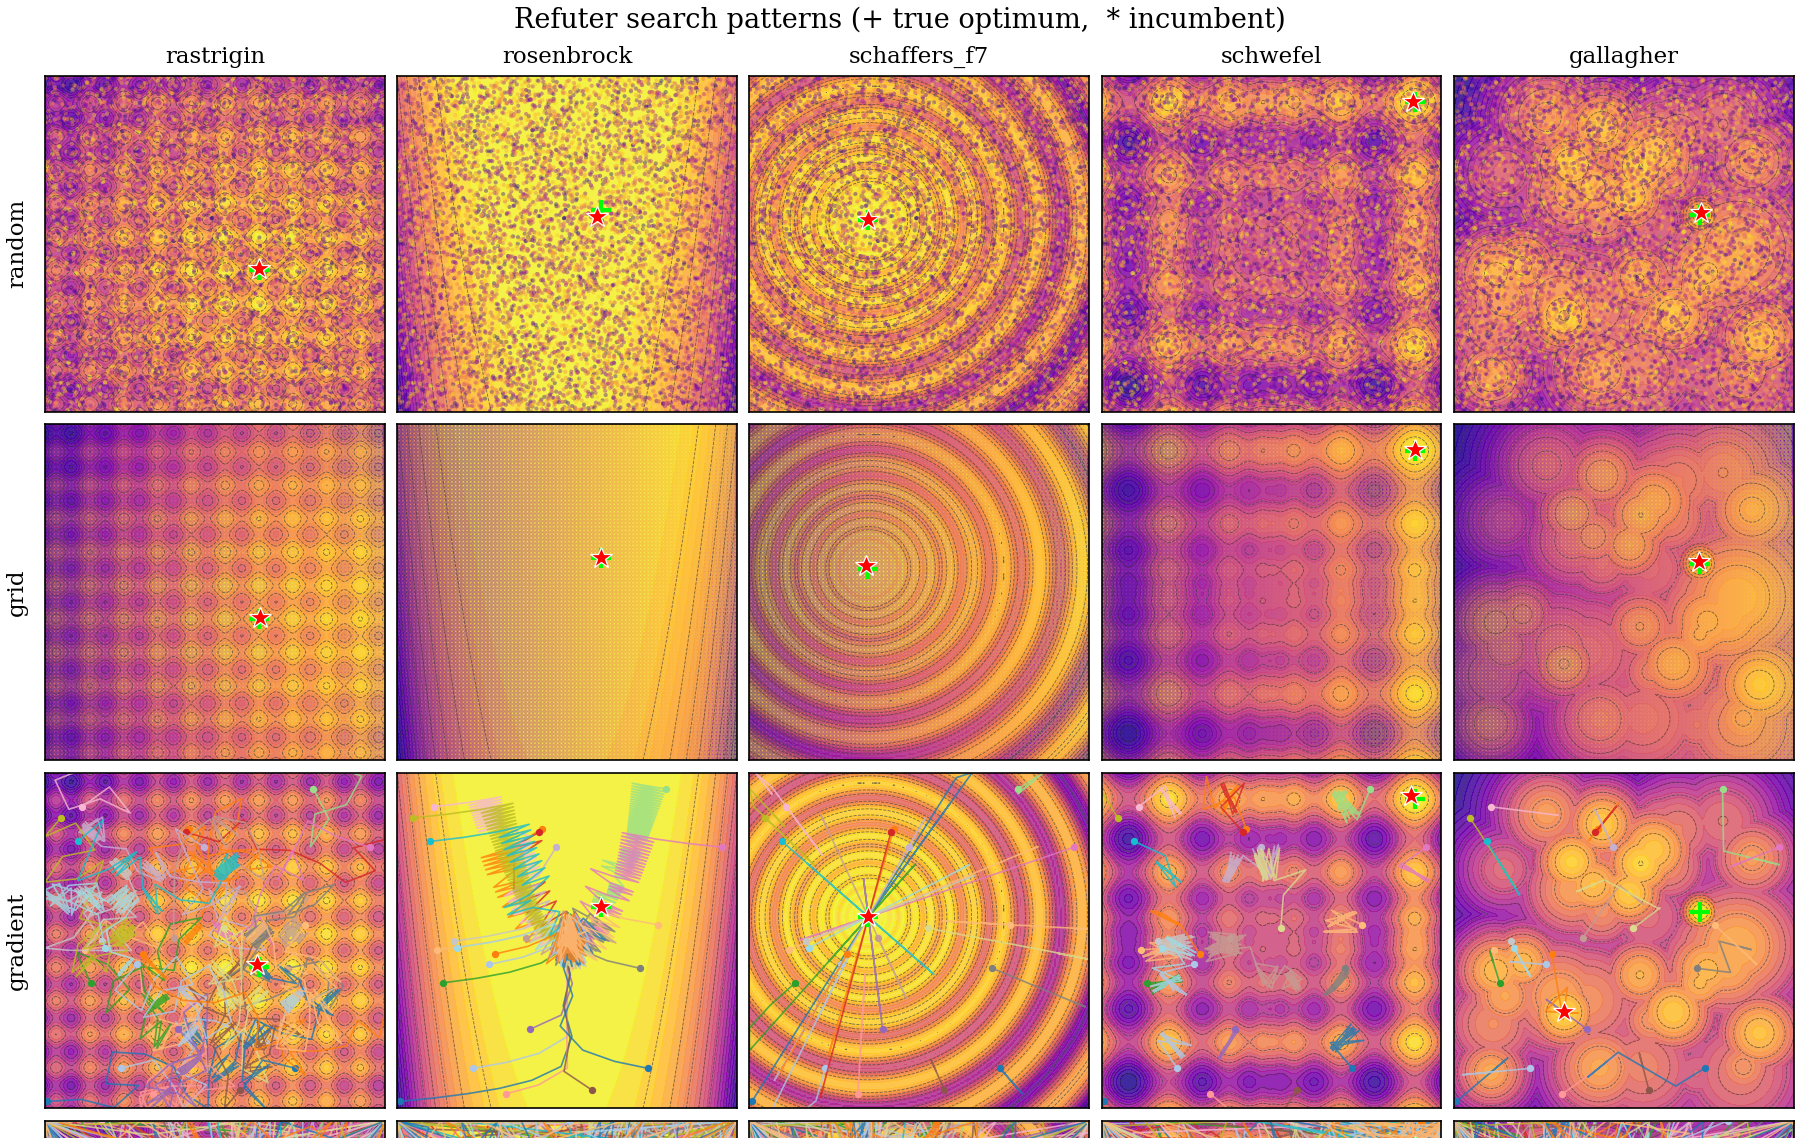
\includegraphics[width=0.96\textwidth,height=0.82\textheight,keepaspectratio]{refuter_patterns_top.png}
\end{frame}

\begin{frame}{Refuter search patterns (II): whale, AdaLIPO, DIRECT}
  \centering
  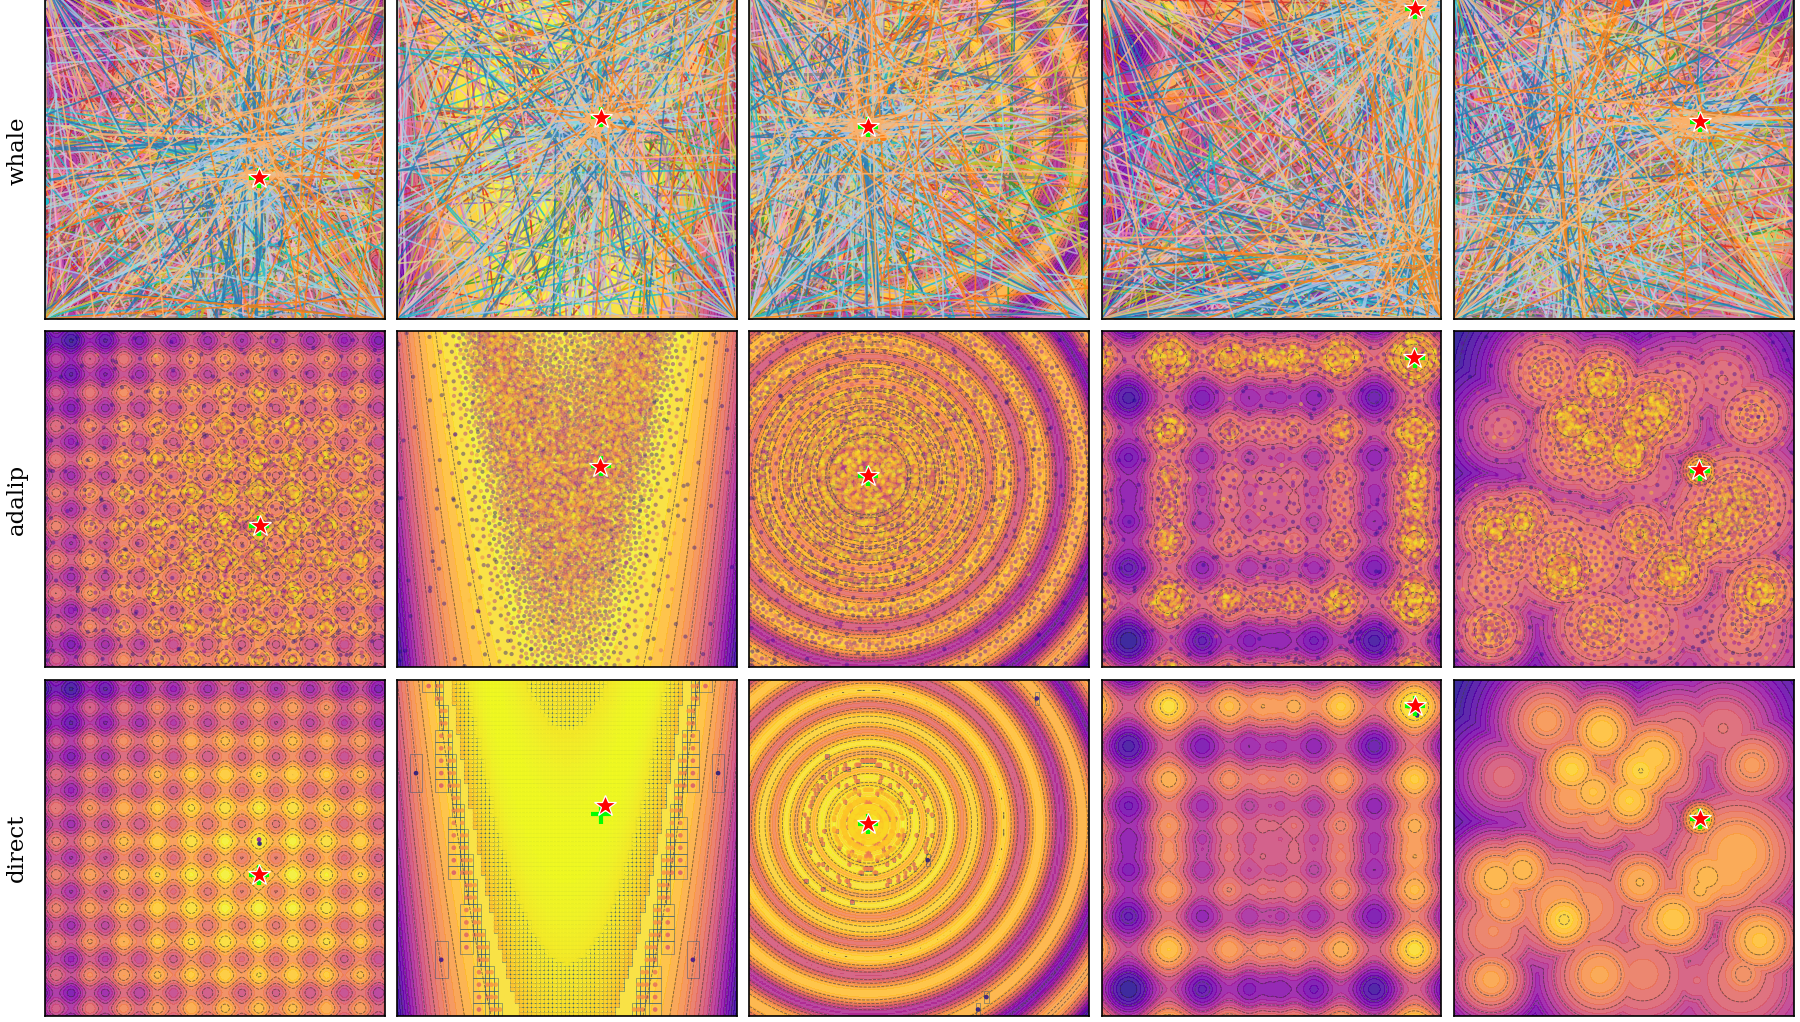
\includegraphics[width=0.96\textwidth,height=0.78\textheight,keepaspectratio]{refuter_patterns_bot.png}\\[1mm]
  {\scriptsize columns: Rastrigin, Rosenbrock, Schaffers~F7, Schwefel, Gallagher}
\end{frame}

\begin{frame}{$\mathrm{LinSwitch}$ certificate portrait}
  \centering
  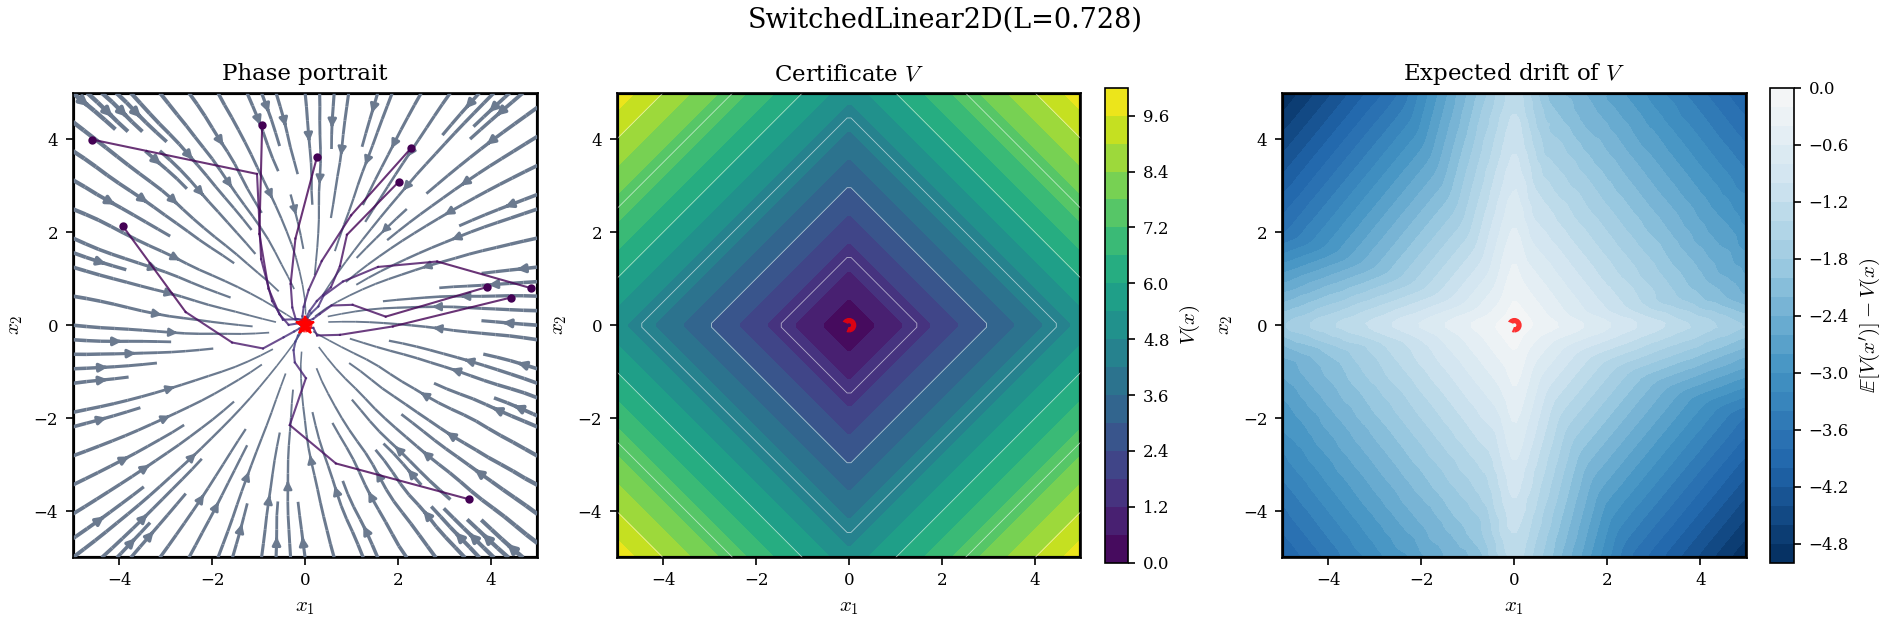
\includegraphics[width=0.8\textwidth,height=0.8\textheight,keepaspectratio]{linear2D_portrait.png}
\end{frame}

\end{document}
